\documentclass[]{book}
\usepackage{lmodern}
\usepackage{amssymb,amsmath}
\usepackage{ifxetex,ifluatex}
\usepackage{fixltx2e} % provides \textsubscript
\ifnum 0\ifxetex 1\fi\ifluatex 1\fi=0 % if pdftex
  \usepackage[T1]{fontenc}
  \usepackage[utf8]{inputenc}
\else % if luatex or xelatex
  \ifxetex
    \usepackage{mathspec}
  \else
    \usepackage{fontspec}
  \fi
  \defaultfontfeatures{Ligatures=TeX,Scale=MatchLowercase}
\fi
% use upquote if available, for straight quotes in verbatim environments
\IfFileExists{upquote.sty}{\usepackage{upquote}}{}
% use microtype if available
\IfFileExists{microtype.sty}{%
\usepackage{microtype}
\UseMicrotypeSet[protrusion]{basicmath} % disable protrusion for tt fonts
}{}
\usepackage[margin=1in]{geometry}
\usepackage{hyperref}
\hypersetup{unicode=true,
            pdftitle={SOC 4650/5650 User's Guide},
            pdfauthor={Christopher Prener, Ph.D.},
            pdfborder={0 0 0},
            breaklinks=true}
\urlstyle{same}  % don't use monospace font for urls
\usepackage{natbib}
\bibliographystyle{apalike}
\usepackage{color}
\usepackage{fancyvrb}
\newcommand{\VerbBar}{|}
\newcommand{\VERB}{\Verb[commandchars=\\\{\}]}
\DefineVerbatimEnvironment{Highlighting}{Verbatim}{commandchars=\\\{\}}
% Add ',fontsize=\small' for more characters per line
\usepackage{framed}
\definecolor{shadecolor}{RGB}{248,248,248}
\newenvironment{Shaded}{\begin{snugshade}}{\end{snugshade}}
\newcommand{\KeywordTok}[1]{\textcolor[rgb]{0.13,0.29,0.53}{\textbf{{#1}}}}
\newcommand{\DataTypeTok}[1]{\textcolor[rgb]{0.13,0.29,0.53}{{#1}}}
\newcommand{\DecValTok}[1]{\textcolor[rgb]{0.00,0.00,0.81}{{#1}}}
\newcommand{\BaseNTok}[1]{\textcolor[rgb]{0.00,0.00,0.81}{{#1}}}
\newcommand{\FloatTok}[1]{\textcolor[rgb]{0.00,0.00,0.81}{{#1}}}
\newcommand{\ConstantTok}[1]{\textcolor[rgb]{0.00,0.00,0.00}{{#1}}}
\newcommand{\CharTok}[1]{\textcolor[rgb]{0.31,0.60,0.02}{{#1}}}
\newcommand{\SpecialCharTok}[1]{\textcolor[rgb]{0.00,0.00,0.00}{{#1}}}
\newcommand{\StringTok}[1]{\textcolor[rgb]{0.31,0.60,0.02}{{#1}}}
\newcommand{\VerbatimStringTok}[1]{\textcolor[rgb]{0.31,0.60,0.02}{{#1}}}
\newcommand{\SpecialStringTok}[1]{\textcolor[rgb]{0.31,0.60,0.02}{{#1}}}
\newcommand{\ImportTok}[1]{{#1}}
\newcommand{\CommentTok}[1]{\textcolor[rgb]{0.56,0.35,0.01}{\textit{{#1}}}}
\newcommand{\DocumentationTok}[1]{\textcolor[rgb]{0.56,0.35,0.01}{\textbf{\textit{{#1}}}}}
\newcommand{\AnnotationTok}[1]{\textcolor[rgb]{0.56,0.35,0.01}{\textbf{\textit{{#1}}}}}
\newcommand{\CommentVarTok}[1]{\textcolor[rgb]{0.56,0.35,0.01}{\textbf{\textit{{#1}}}}}
\newcommand{\OtherTok}[1]{\textcolor[rgb]{0.56,0.35,0.01}{{#1}}}
\newcommand{\FunctionTok}[1]{\textcolor[rgb]{0.00,0.00,0.00}{{#1}}}
\newcommand{\VariableTok}[1]{\textcolor[rgb]{0.00,0.00,0.00}{{#1}}}
\newcommand{\ControlFlowTok}[1]{\textcolor[rgb]{0.13,0.29,0.53}{\textbf{{#1}}}}
\newcommand{\OperatorTok}[1]{\textcolor[rgb]{0.81,0.36,0.00}{\textbf{{#1}}}}
\newcommand{\BuiltInTok}[1]{{#1}}
\newcommand{\ExtensionTok}[1]{{#1}}
\newcommand{\PreprocessorTok}[1]{\textcolor[rgb]{0.56,0.35,0.01}{\textit{{#1}}}}
\newcommand{\AttributeTok}[1]{\textcolor[rgb]{0.77,0.63,0.00}{{#1}}}
\newcommand{\RegionMarkerTok}[1]{{#1}}
\newcommand{\InformationTok}[1]{\textcolor[rgb]{0.56,0.35,0.01}{\textbf{\textit{{#1}}}}}
\newcommand{\WarningTok}[1]{\textcolor[rgb]{0.56,0.35,0.01}{\textbf{\textit{{#1}}}}}
\newcommand{\AlertTok}[1]{\textcolor[rgb]{0.94,0.16,0.16}{{#1}}}
\newcommand{\ErrorTok}[1]{\textcolor[rgb]{0.64,0.00,0.00}{\textbf{{#1}}}}
\newcommand{\NormalTok}[1]{{#1}}
\usepackage{longtable,booktabs}
\usepackage{graphicx,grffile}
\makeatletter
\def\maxwidth{\ifdim\Gin@nat@width>\linewidth\linewidth\else\Gin@nat@width\fi}
\def\maxheight{\ifdim\Gin@nat@height>\textheight\textheight\else\Gin@nat@height\fi}
\makeatother
% Scale images if necessary, so that they will not overflow the page
% margins by default, and it is still possible to overwrite the defaults
% using explicit options in \includegraphics[width, height, ...]{}
\setkeys{Gin}{width=\maxwidth,height=\maxheight,keepaspectratio}
\usepackage[normalem]{ulem}
% avoid problems with \sout in headers with hyperref:
\pdfstringdefDisableCommands{\renewcommand{\sout}{}}
\IfFileExists{parskip.sty}{%
\usepackage{parskip}
}{% else
\setlength{\parindent}{0pt}
\setlength{\parskip}{6pt plus 2pt minus 1pt}
}
\setlength{\emergencystretch}{3em}  % prevent overfull lines
\providecommand{\tightlist}{%
  \setlength{\itemsep}{0pt}\setlength{\parskip}{0pt}}
\setcounter{secnumdepth}{5}
% Redefines (sub)paragraphs to behave more like sections
\ifx\paragraph\undefined\else
\let\oldparagraph\paragraph
\renewcommand{\paragraph}[1]{\oldparagraph{#1}\mbox{}}
\fi
\ifx\subparagraph\undefined\else
\let\oldsubparagraph\subparagraph
\renewcommand{\subparagraph}[1]{\oldsubparagraph{#1}\mbox{}}
\fi

%%% Use protect on footnotes to avoid problems with footnotes in titles
\let\rmarkdownfootnote\footnote%
\def\footnote{\protect\rmarkdownfootnote}

%%% Change title format to be more compact
\usepackage{titling}

% Create subtitle command for use in maketitle
\newcommand{\subtitle}[1]{
  \posttitle{
    \begin{center}\large#1\end{center}
    }
}

\setlength{\droptitle}{-2em}
  \title{SOC 4650/5650 User's Guide}
  \pretitle{\vspace{\droptitle}\centering\huge}
  \posttitle{\par}
  \author{Christopher Prener, Ph.D.}
  \preauthor{\centering\large\emph}
  \postauthor{\par}
  \predate{\centering\large\emph}
  \postdate{\par}
  \date{2017-02-04}

\usepackage{booktabs}

\begin{document}
\maketitle

{
\setcounter{tocdepth}{1}
\tableofcontents
}
\chapter*{Preface}\label{preface}
\addcontentsline{toc}{chapter}{Preface}

This text is a companion document for \textbf{SOC 4650/5650 -
Introduction to Geographic Information Sciences}. It is designed to help
you be \emph{successful} in this course. The idea behind a course
\textbf{User's Guide} is to create a reference for many of the
intangible, subtle or disparate skills and ideas that contribute to
being a successful researcher. In creating a \textbf{User's Guide}, I
draw inspiration from the work of Donald Knuth.\footnote{\href{https://en.wikipedia.org/wiki/Donald_Knuth}{Donald
  Knuth} is the developer of
  \href{https://en.wikipedia.org/wiki/TeX}{TeX}, a computer typesetting
  system that is widely used today for scientific publishing in the form
  of \href{https://en.wikipedia.org/wiki/LaTeX}{LaTeX}. He also
  established the concept of
  \href{https://en.wikipedia.org/wiki/Literate_programming}{literate
  programming}, which forms the basis of some of the practices we will
  follow with Stata this semester.} Knuth has discussed his experiences
in designing new software languages, nothing that the developer of a new
language

\begin{quote}
\ldots{}must not only be the implementer and the first large-scale user;
the designer should also write the first user manual\ldots{} If I had
not participated fully in all these activities, literally hundreds of
improvements would never have been made, because I would never have
thought of them or perceived why they were important\ldots{}
\end{quote}

While there is nothing particularly new about what I am writing here,
and I am certainly not developing a new language for computing, the goal
of the \textbf{User's Guide} remains similar to Knuth's experience. By
distilling some of key elements for making a successful transition to
being a \emph{professional developer} of knowledge rather than a
\emph{casual consumer}, I hope to both improve the course experience
itself and also create an environment that fosters a successful learning
experience for you.

If you read through the course objectives included in the syllabus, you
will note that creating maps is only one of them. As much as this is a
GIS course, it is a course in research methods. In particular, we are
concerned with \emph{high quality} research methods and the
\emph{process} of conducting research. We therefore focus on a
combination of mental habits and technical practices that make you a
successful researcher. Some of the skills and techniques that we will
discuss this semester are not taught as often in graduate programs.
Instead, they are often the products of ``learning the hard way''. These
``habits of mind and habits of method'' are broadly applicable across
methodologies and disciplines.

\section*{License}\label{license}
\addcontentsline{toc}{section}{License}

Copyright © 2016-2017 \href{http://chrisprener.net}{Christopher G.
Prener}

This work is licensed under a Creative Commons Attribution 4.0
International License.

\chapter{Getting Started}\label{gettingStarted}

Before you begin the semester, there are a number of things that I
recommend that you do to help set yourself up for success. Before you do
\emph{anything} else, you should read through the
\href{}{\textbf{Syllabus}} and the \href{}{\textbf{Reading List}}. Make
sure you have a good sense of what is \emph{required} for the course. If
you have questions, bring them to the first day of class!

\section{Prep Your Computer}\label{prep-your-computer}

Before you do anything else for this course, make sure you get your
computer ready for the work you are about to undertake:

\begin{enumerate}
\def\labelenumi{\arabic{enumi}.}
\tightlist
\item
  Make sure your operating system is up-to-date. If you are able, I
  would also recommend upgrading your computer to the most recent
  release of its operating system that the computer can run.
\item
  We'll be sharing computer files throughout the semester, so you should
  ensure that you have functioning anti-virus software and that it is
  up-to-date.
\item
  You'll also need to download files, so you'll need to make sure you
  have some free space on your hard drive. If you have less than 10GB of
  free space, you should de-clutter!
\item
  Make sure you know how to access your computer's file management
  system.

  \begin{itemize}
  \tightlist
  \item
    On macOS, this means being comfortable with Finder.app.
  \item
    On Windows, this means being comfortable with Windows Explorer.
  \end{itemize}
\end{enumerate}

This of course assumes that you own a computer. Owning a computer is not
required for this course. All students who are enrolled in SOC 4650 or
SOC 5650 will be given 24-hour swipe access (\emph{just what you always
wanted!}) to Morrissey Hall to facilitate access to lab computers.

\section{Create Accounts}\label{create-accounts}

There are two major web services that we will use this semester, and
you'll need to create accounts for both:

\begin{itemize}
\tightlist
\item
  \textbf{GitHub} - you can sign-up at
  \href{https://github.com}{GitHub.com}. Once you've signed up, fill out
  your profile, set-up
  \href{https://help.github.com/articles/about-two-factor-authentication/}{two-factor
  authentication}, and let Chris know (via
  \href{mailto:prenercg@slu.edu}{email}) what your user name is. Once he
  has it, he can add you to the
  \href{https://github.com/slu-soc5650}{SOC 4650/5650} organization.
\item
  \textbf{Slack} - you can ask Chris (via
  \href{mailto:prenercg@slu.edu}{email}) for an invitation to sign-up
  for our team. Once the sign-up process is complete, you can log-in by
  going to our team's \href{https://slu-soc5650.slack.com}{Slack site}.
  Fill out your profile, set-up
  \href{https://get.slack.help/hc/en-us/articles/204509068-Set-up-two-factor-authentication}{two-factor
  authentication}, and change your timezone.
\end{itemize}

\section{Download and Install
Software}\label{download-and-install-software}

There are a number of software applications that we will use this
semester. Most of them are free, and I recommend downloading those free
ones right away. All of these applications are available for macOS and
Windows.

\begin{itemize}
\tightlist
\item
  \textbf{Atom} - Atom is a flexible, open-source text editor that is
  produced by GitHub. You can download it from Atom's
  \href{https://atom.io}{website}.
\item
  \textbf{GitHub Desktop} - GitHub makes a desktop client that you can
  use to easily interact with repositories that are stored on the site.
  You can download it from GitHub's
  \href{https://desktop.github.com}{website} after you sign-up for an
  account there. You'll need that account information to complete the
  desktop client's set-up process.
\item
  \textbf{Slack} - Slack has a number of applications for desktop and
  mobile operating systems. I recommend downloading Slack on your
  personal computer, and optionally installing it on your mobile device
  as well. You can download their desktop applications from their
  \href{https://slack.com/downloads}{website} and the mobile
  applications from your App Store.
\end{itemize}

\subsection*{\texorpdfstring{For Graduate Students
\emph{only}}{For Graduate Students only}}\label{for-graduate-students-only}
\addcontentsline{toc}{subsection}{For Graduate Students \emph{only}}

If your computer meets the
\href{http://desktop.arcgis.com/en/arcmap/10.3/get-started/system-requirements/arcgis-desktop-system-requirements.htm}{operating
system requirements} for ArcGIS and you think you'd benefit from having
access to the software at home, let Chris know (via
\href{mailto:prenercg@slu.edu}{email}).

If you are in the Public and Social Policy Ph.D.~program and your
computer meets the
\href{http://www.stata.com/support/faqs/windows/hardware-requirements/}{hardware}
and
\href{http://www.stata.com/products/compatible-operating-systems/}{software}
requirements for Stata, you should consider
\href{https://www.stata.com/order/new/edu/gradplans/student-pricing/}{purchasing
it} for yourself. I recommend purchasing a perpetual license for
Stata/IC. This is the most cost-effective solution for typical students.

\section{Buy Course Materials}\label{buy-course-materials}

\subsection*{Books}\label{books}
\addcontentsline{toc}{subsection}{Books}

There are three required books for this course:

\begin{enumerate}
\def\labelenumi{\arabic{enumi}.}
\tightlist
\item
  Brewer, Cynthia. 2015. \emph{Designing Better Maps: A Guide for GIS
  Users}. Redlands, CA: ESRI Press. ISBN-13: 978-1589484405; List Price:
  \$59.99; ebook versions available.
\item
  Gorr, Wilpen L. and Kristen S. Kurland. 2013. \emph{GIS Tutorial 1:
  Basic Workbook}. 10.3.x edition. Redlands, CA: ESRI Press. ISBN-13:
  978-1589484566; List Price: \$79.99; ebook versions available.
\item
  Thomas, Christopher and Nancy Humenik-Sappington. 2009. \emph{GIS for
  Decision Support and Public Policy Making}. Redlands, CA: ESRI Press.
  ISBN-13: 978-1589482319; List Price: \$24.95.
\end{enumerate}

There is one additional book that is optional:

\begin{itemize}
\tightlist
\item
  Mitchell, Michael N. 2010. \emph{Data Management Using Stata: A
  Practical Handbook}. College Station, TX: Stata Press. ISBN-13:
  978-1597180764; List Price: \$48.00.
\end{itemize}

Buying Mitchell (2010) is \emph{highly} recommended for graduate
students who will continue using Stata in the future and those who are
concerned about the command-line interface. I recommend waiting for a
week or two before purchasing this.

\subsection*{External Media}\label{external-media}
\addcontentsline{toc}{subsection}{External Media}

You will need a USB external storage device (either an external hard
drive or a thumb-style drive) that has at least 20GB of storage
capacity. This will be used for storing spatial data for this course.

\section{Download Course Data}\label{download-course-data}

Mots of the course data is available for download via Dropbox in a
single \texttt{.zip} file. If you want, you can let Chris know (via
\href{mailto:prenercg@slu.edu}{email}) that you'd like to download these
data before the beginning of the semester. Once you download them,
extract the data from the \texttt{.zip} file and transfer them to your
external storage device.

\chapter{Approaching this Course}\label{approaching-this-course}

Students have varying experiences learning GIS techniques. For some, the
spatial logic and programming that are the foundation for GIS methods
come naturally. For others, being introduced to these concepts can be an
anxiety producing experience. I am fond the phrase ``your mileage will
vary'' for describing these differences - no two students have the exact
same experience taking a methods course.

\section{Zen and the Art of Data
Analysis}\label{zen-and-the-art-of-data-analysis}

One of the biggest challenges with this course can be controlling the
anxiety that comes along with learning new skills. ArcGIS processes,
Markdown syntax, and Stata commands can seem like foreign alphabets at
first. Debugging Stata do-files can be both challenging and a large time
suck, in part because you are not yet fluent with this language. Imagine
trying to proofread a document written in a language that you only know
in a cursory way but where you must find minute inconsistencies like
misplaced commas.

For this reason, I also think it is worth reminding you that many
students in the social sciences struggle with quantitative methods at
first. It is normal to find this challenging and frustrating. I find
that students who can recognize when they are beginning to go around in
circles are often the most successful at managing the issues that will
certainly arise during this course. Recognizing the signs that you are
starting to spin your wheels and taking either ten minutes, an hour or
two, or a day away from GIS coursework is often a much better approach
than trying to power through problems.

\section{An Apple a Day}\label{an-apple-a-day}

Being able to walk away from an assignment for a day requires excellent
time management. If you are waiting until the night before or the day of
an assignment's due day to begin it, you give yourself little room for
errors. I recommend approaching this course in bite size chunks - a
little each day. The most successful students do not do all of their
reading, homework, and studying in a single sitting. I find that this
approach not only creates unnecessary anxiety around assignments, it
also dramatically limits the amount of course material you can absorb.
Keep in mind that I expect the \emph{median} student to spend
approximately six hours on work for this class each week (twice the
amount of in-class time).

A sample approach to the class might look something like this:

\begin{itemize}
\tightlist
\item
  Tuesday: class
\item
  Wednesday: finish lab
\item
  Thursday: Start problem set
\item
  Friday: Finish problem set
\item
  Saturday: First reading
\item
  Monday: Second reading
\end{itemize}

\section{Reading with Purpose}\label{reading-with-purpose}

The book and article \textbf{reading assignments} for this course are
different from most of the other reading you will do in your graduate
program because they are often very technical. Students who are most
successful in this course read twice. Read the first time to expose
yourself to the material, then take a break from the reading. During
this first read, I don't recommend trying to complete the example
problems or programming examples. Focus on the \emph{big picture} - what
are the concepts and ideas that these readings introduce?

During the second read, try to focus in in the \emph{details} - what are
the technical details behind the big picture concepts? I recommend doing
this second read with your computer open. Follow along with the examples
and execute as much of them as you can. By using this second read
through as a way to test the waters and experiment with the week's
content, you can come into the lecture better prepared to take full
advantage of the class period. Students who follow this approach are
able make important connections and focus on the essential details
during lectures because it is their third time being exposed to the
course material. They are also in a much stronger position to ask
questions.

\section{Active Lectures and Labs}\label{active-lectures-and-labs}

During \textbf{lectures}, I introduce many of the same topics that your
readings cover. This again is intentional - it gives you yet another
exposure to concepts and techniques that are central to geospatial
science. One mistake students sometimes make is focusing on the details
of \emph{how} to do a particular task rather than focusing on
\emph{when} a task should be done. If you know when a task is needed but
cannot remember how to do it in Stata or ArcGIS, you can look this
information up. Conversely, detailed notes on executing Stata commands
may not be helpful if you are unsure when to use a particular skill.
There is no penalty in this course for not knowing how to execute a
command from memory; this is what reference materials are for. The most
successful students will therefore focus on \emph{when} a particular
skill is warranted first before focusing on \emph{how} to execute that
skill

Getting experience with executing tasks is the purpose of the
\textbf{lab exercises}. Time for beginning these exercises is given at
the end of each class meeting, and replication files will be posted on
GitHub for each lab.

\section{Typefaces and Examples}\label{typefaces-and-examples}

\subsection{Typefaces and Fonts}\label{typefaces-and-fonts}

Technical publications that describe scientific computing processes use
a \texttt{monospaced\ typewriter\ style\ typeface} to refer to commands
(inputs) and results (outputs). In some documents, like lecture slides
and cheat-sheets, I may highlight a command by using a to increase the
visibility of the command name itself.

The \texttt{typewriter\ typeface} is also used to refer to filenames
(e.g. \texttt{auto.dta}) or filepaths (e.g.
\texttt{C:\textbackslash{}Users\textbackslash{}JSmith\textbackslash{}Desktop}).
Finally, we will use the \texttt{typewriter\ typeface} to refer to
GitHub repositories (e.g. \texttt{Core-Documents}, the repository that
contains this file).

Technical publications use \emph{italicized text} to refer to text that
is meant to be replaced. These references will typically appear in a
\texttt{typewriter\ typeface} since they are often part of commands. For
example, \texttt{describe\ varname} (with \texttt{varname}
\emph{italicized}) indicates that you should replace the text
\texttt{varname} with the appropriate variable name from your dataset.

These publications also use a sans serif typeface to refer to areas of
the user interface, menu items, and buttons. I cannot replicate that
here because of the publishing software that I use, but you'll notice
this text in course documents. We will therefore use the
\texttt{typewriter\ typeface} in the User Guide to identify these same
features.

Technical documents also use a sans serif or \texttt{typewriter}
typeface to refer to keyboard keys (e.g. \texttt{Crtl+C}) where the plus
sign (\texttt{+}) indicates that you should press multiple keys at the
same time. A sans serif typeface combined with a right facing
triangle-style arrow (\texttt{\textgreater{}}) is used to refer to
actions that require clicking through a hierarchy of menus or windows
(e.g. \texttt{File\ \textgreater{}\ Save}).

\subsection{Examples}\label{examples}

Throughout the semester, I will give you examples both in lecture slides
and in an example do-file. Examples in lectures and course documents can
be easily identified by their use of the \texttt{typewriter\ typeface}:

\begin{verbatim}
. summarize mpg
    Variable |        Obs        Mean    Std. Dev.       Min        Max
-------------+---------------------------------------------------------
         mpg |         74     21.2973    5.785503         12         41
\end{verbatim}

Examples will almost always use the file \texttt{census.dta}, which
comes pre-installed with Stata. To open it, use the \texttt{sysuse}
command: \texttt{sysuse\ census.dta,\ clear}. This allows you to easily
recreate examples by minimizing dependencies within do-files.

\chapter{\texorpdfstring{``Good Enough'' Research
Practices}{Good Enough Research Practices}}\label{good-enough-research-practices}

This section introduces some of the core concepts that we will emphasize
in this course throughout the semester. The title takes inspiration from
a recent article titled \href{https://arxiv.org/abs/1609.00037}{``Good
Enough Practices in Scientific Computing''}\footnote{Wilson, G., Bryan,
  J., Cranston, K., Kitzes, J., Nederbragt, L. and Teal, T.K., 2016.
  Good Enough Practices in Scientific Computing. \emph{arXiv preprint
  arXiv:1609.00037.}}. The authors note in their introduction that
scientific computing advice can sometimes be both overwhelming and
focused on tools that are inaccessible to many analysts. Their goal, and
the goal of this course, is to de-mystify the simplist tools that enable
researchers to streamline their workflows:

\begin{quote}
Our intended audience is researchers who are working alone or with a
handful of collaborators on projects lasting a few days to a few months,
and who are ready to move beyond emailing themselves a spreadsheet named
\texttt{results-updated-3-revised.xlsx} at the end of the
workday\ldots{}Many of our recommendations are for the benefit of the
collaborator every researcher cares about most: their future self.
\end{quote}

I would argue that the skills they describe are useful beyond just a few
months. Indeed, most of the skills here can dramatically improve
students' dissertation experiences:

\begin{quote}
Most importantly, these practices make researchers more productive
individually by enabling them to get more done in less time and with
less pain. They also accelerate research as a whole by making
computational work (which increasingly means all work) more
reproducible. But progress will not happen by itself. Universities and
funding agencies need to support training for researchers in the use of
these tools. Such investment will improve confidence in the results of
computational work and allow us to make more rapid progress on important
research questions.
\end{quote}

While much of what we will talk about in this course is aimed at
supporting your work, there are benefits that extend beyond your
dissertation or your research projects. These benefits, which include
developing sustainable workflows and structuring the way you interact
with your own computer, can make everyday computing practices like
checking email or organizing files an easier, more structured process.

\section{Reproducibility}\label{reproducibility}

One of the mantras of this course is our emphasis on reproducibility.
The unifying feature of all of the ``good enough'' research practices
discussed below is that they contribute to a more reproducible research
product.

Reproducibility is very much in vogue right now for number of reasons.
\href{http://science.sciencemag.org/content/349/6251/aac4716}{Assessments
of studies in psychology}\footnote{Open Science Collaboration, 2015.
  Estimating the reproducibility of psychological science.
  \emph{Science}, 349(6251), p.aac4716.}, for example, have found weaker
on average effect sizes and far fewer statistically significant results
than the initial studies reported. There have also been high profile
instances of falsified research, including
\href{http://nymag.com/scienceofus/2015/05/how-a-grad-student-uncovered-a-huge-fraud.html}{research
by a graduate student at UCLA}. This particular instance of fraud was
identified by graduate students intent on replicating the original
study.

At the same time, there is a recognition that the skills necessary for
producing reproducible research are not being fostered in academic
disciplines and graduate programs. Thus one of the goals of this course,
and this \textbf{User's Guide} in particular, is to help develop a
working knowledge of many of these skills.

One challenge, however, is that reproducibility does not have a
consistent definition. Some researchers use the term to narrowly refer
to code that can execute without alteration on a person's computer.
Others use it to refer to research designs that can be replicated by
other researchers. Still others discuss reproducibility as the ability
to obtain a similar set of results or draw similar inferences from
identical research designs.

When we talk about reproducibility in this class. We'll be primarily
concerned with \textbf{methods reproducibility}:

\begin{quote}
the ability to implement, as exactly as possible, the experimental and
computational procedures, with the same data and tools, to obtain the
same results.\footnote{Goodman, S.N., Fanelli, D. and Ioannidis, J.P.,
  2016. What does research reproducibility mean?. \emph{Science
  translational medicine}, 8(341), pp.341ps12-341ps12.}
\end{quote}

Methods reproducibility in GISc means that other analysts have full
access to both the original data and the steps used to render those
original data into a final research product, such as a set of maps. This
is increasingly seen not just a matter of good research methodology, but
as a matter of research ethics as well. Being able to be transparent
with research decreases the potential for cases like the
\href{http://nymag.com/scienceofus/2015/05/how-a-grad-student-uncovered-a-huge-fraud.html}{fraudulent
dissertation research conducted by a UCLA graduate student named Michael
LaCour}. It was the efforts of
\href{https://fivethirtyeight.com/features/how-two-grad-students-uncovered-michael-lacour-fraud-and-a-way-to-change-opinions-on-transgender-rights/}{two
Stanford graduate students who wanted to reproduce LaCour's findings}
that ultimately led to the identification of problematic work.

For GISc, methods reproducibility is derived from a number of sources.
The first source is the use of \textbf{computer code} for working with
data. Rather than making manual changes to tabular data in a spreadsheet
application like Microsoft Excel, computer code provides detailed
records of each individual alterations. Code can be used execute tasks
repeatedly, meaning that errors can be easily fixed if they are
discovered an hour, a day, a week, or a month later. During this
semester, we'll use Stata's programming language to execute reproducible
data cleaning processes.

Operations in ArcGIS can also be scripted using the programming language
\href{https://www.python.org}{Python}. Python is an open-source language
that is widely used by data analysts and computer programmers. We will
not learn
\href{http://pro.arcgis.com/en/pro-app/arcpy/get-started/what-is-arcpy-.htm}{ArcPy},
the library of Python commands for ArcGIS, this semester. However, it is
important to know that many of the things we will learn this semester
\emph{can} be scripted, dramatically increasing the reproducibility of
your work.\footnote{For those of you who are interested, we'll be
  providing Python/ArcPy examples for many of the ArcGIS tasks we learn
  this semester. These will be available on GitHub in the \texttt{ArcPy}
  repository for those of you interested in expanding your knowledge.}

Since we won't focus on scripting for ArcGIS this semester, much of the
work we will do will be done manually. This means that no record exists
of the changes we make or the steps that we take to complete a task.
From a reproducibility standpoint, this is problematic. Even if we were
scripting our work in ArcGIS, there are often aspects of projects that
must be completed manually. In GISc, this often arises in initial steps
like download data or in the production of final map products, which
often require using graphic design software.

The second source of reproducibility in GISc is therefore derived from
the \textbf{documentation} that we create to accompany our research
products. These documents outline where our data originated (GIS
metadata files), what specific variables mean (a codebook), what steps
were taken to create specific maps (a research log), and how our data
files are organized (a metadictionary).

Our code can also be used as documentation if it is written using
\href{https://en.wikipedia.org/wiki/Literate_programming}{literate
programming} techniques. In Stata, these techniques produce well
annotated output that ``weaves'' together code, output, and narrative
text that describes the function of the code and the results of the
output.

The third and final primary source of reproducibility in GISc is derived
from our \textbf{organizational approach} to our work. GISc projects can
require many gigabytes of data spread across dozens or even hundreds of
files, feature classes, and databases. A disorganized file system can
make replicating your work difficult if not impossible. Much of the
research practices discussed in the remainder of this section are aimed
at supporting one or more of these three major sources of
reproducibility.

\section{Thinking in Workflows}\label{thinking-in-workflows}

One way to increase the reproducibility of a project is to approach each
and every task with purposeful organization and thoughtfulness.
\textbf{Workflows} are the processes that we use to approach a given
task. Think of checking your email. You (hopefully!) follow a series of
steps when you check your email that help you organize your inbox. When
I check my email for the first time each day, my workflow looks
something like this:

\begin{enumerate}
\def\labelenumi{\arabic{enumi}.}
\tightlist
\item
  Delete junk mail
\item
  Read and then delete New York Times and Washington Post morning
  newsletters
\item
  Read and then delete SLU Newslink newsletter
\item
  For each remaining email:

  \begin{enumerate}
  \def\labelenumii{\alph{enumii}.}
  \tightlist
  \item
    Respond if response will take less than two minutes and/or
  \item
    forward to task management inbox if email requires an action, or
  \item
    snooze\footnote{Snoozing is a ``magical'' feature of the email
      client that I use - \href{http://sparkmailapp.com}{SparkMail}.}
    the message until ``later today'' or ``tomorrow morning'' if
    response will require more time than currently avaiable.
  \end{enumerate}
\end{enumerate}

In our reading for the first week of classes,
\href{http://www.indiana.edu/~jslsoc/}{Scott Long}\footnote{Long, J.S.,
  2009. \emph{The workflow of data analysis using Stata.} College
  Station, TX: Stata Press.} describes a structured strategy for
approaching statistical research. In Long's model, a data analysis
project consists of four steps: (a) data cleaning, (b) analysis, (c)
presenting results, and (d) protecting files. This is a useful model to
build upon for GISc work, and one that we will discuss over the course
of the semester.

Even more useful, not just for GISc work but for any process, are the
tasks Long lays out for each step in the data analysis workflow:

\begin{enumerate}
\def\labelenumi{\arabic{enumi}.}
\tightlist
\item
  Planning
\item
  Organization
\item
  Documentation
\item
  Execution
\end{enumerate}

A good example of the utility of extending this logic to other workflows
is with the problem sets. The ``typical'' approach students take with
homework assignments is to sit down, open up their software, and start
with question 1. Using Long's four task approach, a workflow-based
strategy to the assignment would involve beginning by reading the
assignment through in its entirety to develop a \textbf{plan} for
approaching it - think about what techniques and skills are needed for
each step. With a plan in place, you can proceed to \textbf{organizing}
yourself for the assignment - identifying and obtaining files that you
will need, creating dedicated directories for saving assignment data,
and getting any necessary software documentation. After pulling together
all of these materials, you are ready to move on to
\textbf{documentation} - setting up your assignment code and output
files, and (later in the course) your research log and meta-dictionary.
Once you are set-up, you would then begin to address individual
assignment questions as part of the \textbf{execution} task.

The goal here is to approach everything you do for research or work with
an element of mindfulness and structure about your process. This mental
model for approaching research supports the creation of
\textbf{reproducible} research products because we approach our work in
a routinized, predictable, organized, and efficient manner. Thinking in
terms of workflows also encourages a greater awareness of the complexity
of tasks, which also helps you plan more accurately for how long a
particular task or project will take.

In reality, there will be multiple workflows that you find yourself
navigating. You will want a structured process not just for approaching
a large spatial research project like the final project, but also a
process for maintaining notes related to a specific assignment, a
process for documenting code, a process for approaching assignments, and
even a process for backing your data up. As you go through the course,
think about how to best integrate these ideas into your work habits.

\section{Course Tools}\label{course-tools}

This course relies on a number of major tools to help us accomplish the
work that we need to do. This makes for a complex learning curve,
particularly at the beginning of the semester. The tools we've selected
for this class have been picked not necessarily because they are the
\emph{easiest} tools to learn, but because they \emph{increase} our
ability to conduct reproducible research.

\subsection{ArcGIS}\label{arcgis}

ArcGIS is the industry standard GIS application suite. Though there are
other tools out there that contain much of the same functionality,
ArcGIS remains the expected skill-set for entry-level GIS jobs in nearly
every sector of the labor market. ArcGIS excels at managing and
manipulating spatial data, and has a wide range of tools for creating
data visualizations that use spatial data. For these reasons, ArcGIS
will occupy a large portion of our time this semester.

ArcGIS has two weaknesses for our purposes. While it can be scripted
using \href{https://www.python.org}{Python}, that functionality is not
placed front and center in the application. It also is difficult to pick
up ArcGIS's Python tools, named
\href{http://pro.arcgis.com/en/pro-app/arcpy/get-started/what-is-arcpy-.htm}{ArcPy},
without some background in GIS more generally. This limits the longterm
reproducibility of the GIS work we'll do this semester since it is
driven by the difficult to reproduce point-and-click user interface.

The second weakness that ArcGIS has is a limited set of tools for
cleaning and manipulating tabular data. Not only are these driven by a
point-and-click user interface, and thus limited in their ability to
achieve reproducibility, but they are cumbersome and lack the power of
other approaches to cleaning data.

\subsection{Stata}\label{stata}

Since ArcGIS is limited in its approach to data cleaning, we will use
\href{http://stata.com}{Stata} instead. Stata is, first and foremost,
statistical software. It has its own programming language and syntax
that can be used not only for statistical purposes but also for cleaning
data. For tabular data, therefore, Stata will become an intermediary
tool between raw data and data that is suitable for mapping.

Our approach to using Stata will involve using a technique I described
above called
\href{https://en.wikipedia.org/wiki/Literate_programming}{literate
programming}. The implementation of literate programming in Stata comes
from a user-written package called
**\href{http://haghish.com/statistics/stata-blog/reproducible-research/markdoc.php}{Markdoc}.
Markdoc allows you to embed text that is formatted using the
\href{https://en.wikipedia.org/wiki/Markup_language}{markup language}
\href{https://daringfireball.net/projects/markdown/}{Markdown}. Markdown
is increasingly being adopted as one of the primary data science writing
tools because it is (a) simple, (b) does not require extensive software
or plugins, and (c) is widely support by applications like \texttt{R}
and GitHub. We'll describe both Markdoc and Markdown further in the
chapter ``Reproducible Do-files''.

\subsection{Atom}\label{atom}

While Stata does have a built-in do-file editor, and you could easily
use it to author code for Stata, writing in an external text editor has
a number of advantages. Atom is a free, highly extensible, and easy to
use text editor. Unlike Stata's do-file editor, it is not tied to a
single application or programming language. And unlike Stata's editor,
it cannot be readily extended, customized, or used for work outside of
Stata.

Atom, on the other hand, offers a large number of user-written packages
that dramatically extend its base capabilities. One of those,
\texttt{language-stata}, gives Atom support for working with Stata's
do-file format. Atom also offers a text expansion tool that will help
you write consistently structured and documented do-files. As we
progress through the semester, we'll also use a number of packages for
writing and previewing Markdown text files. So, while using Atom means
adding an additional tool to your workflow, it also offers a number of
improvements over what Stata comes built in with. We'll describe all of
this further in the chapters on ``Introducing Atom'', ``Introducing
Markdown'', and ``Reproducible Do-files''.

\subsection{GitHub}\label{github}

The final tool we'll use, GitHub and its desktop application GitHub
Desktop, is an exceptionally powerful tool for conducting version
control on an entire directory. This allows you to track changes in
individual files as well as changes that impact an entire sub-folder or
entire project directory. GitHub is increasingly recognized as one of
the key tools available for making research reproducible because it
allows users to maintain logs of every change they make on a project. It
also offers other tools that support project management, including to-do
lists, issue tracking, and even website maintenance. Since GitHub
provides support for the \href{http://geojson.org}{GeoJSON} standard for
storing spatial data, we can store and preview(!) shapefiles on GitHub
as well. GitHub, and the software that powers it called Git, are both
described further in the ``Introduction to GitHub''.

\section{Course Workflow}\label{course-workflow}

One of the largest learning curves with this course is keeping track of
how all of these tools fit together. This process is described in detail
in \href{https://github.com/slu-soc5650/week-02}{Week 2's lecture}, but
what follows is a short description of the ``big picture'' at work here.
As we said above, it is important for you to being thinking in
workflows. We've mapped out the major aspects of our course workflow to
help aid that process:

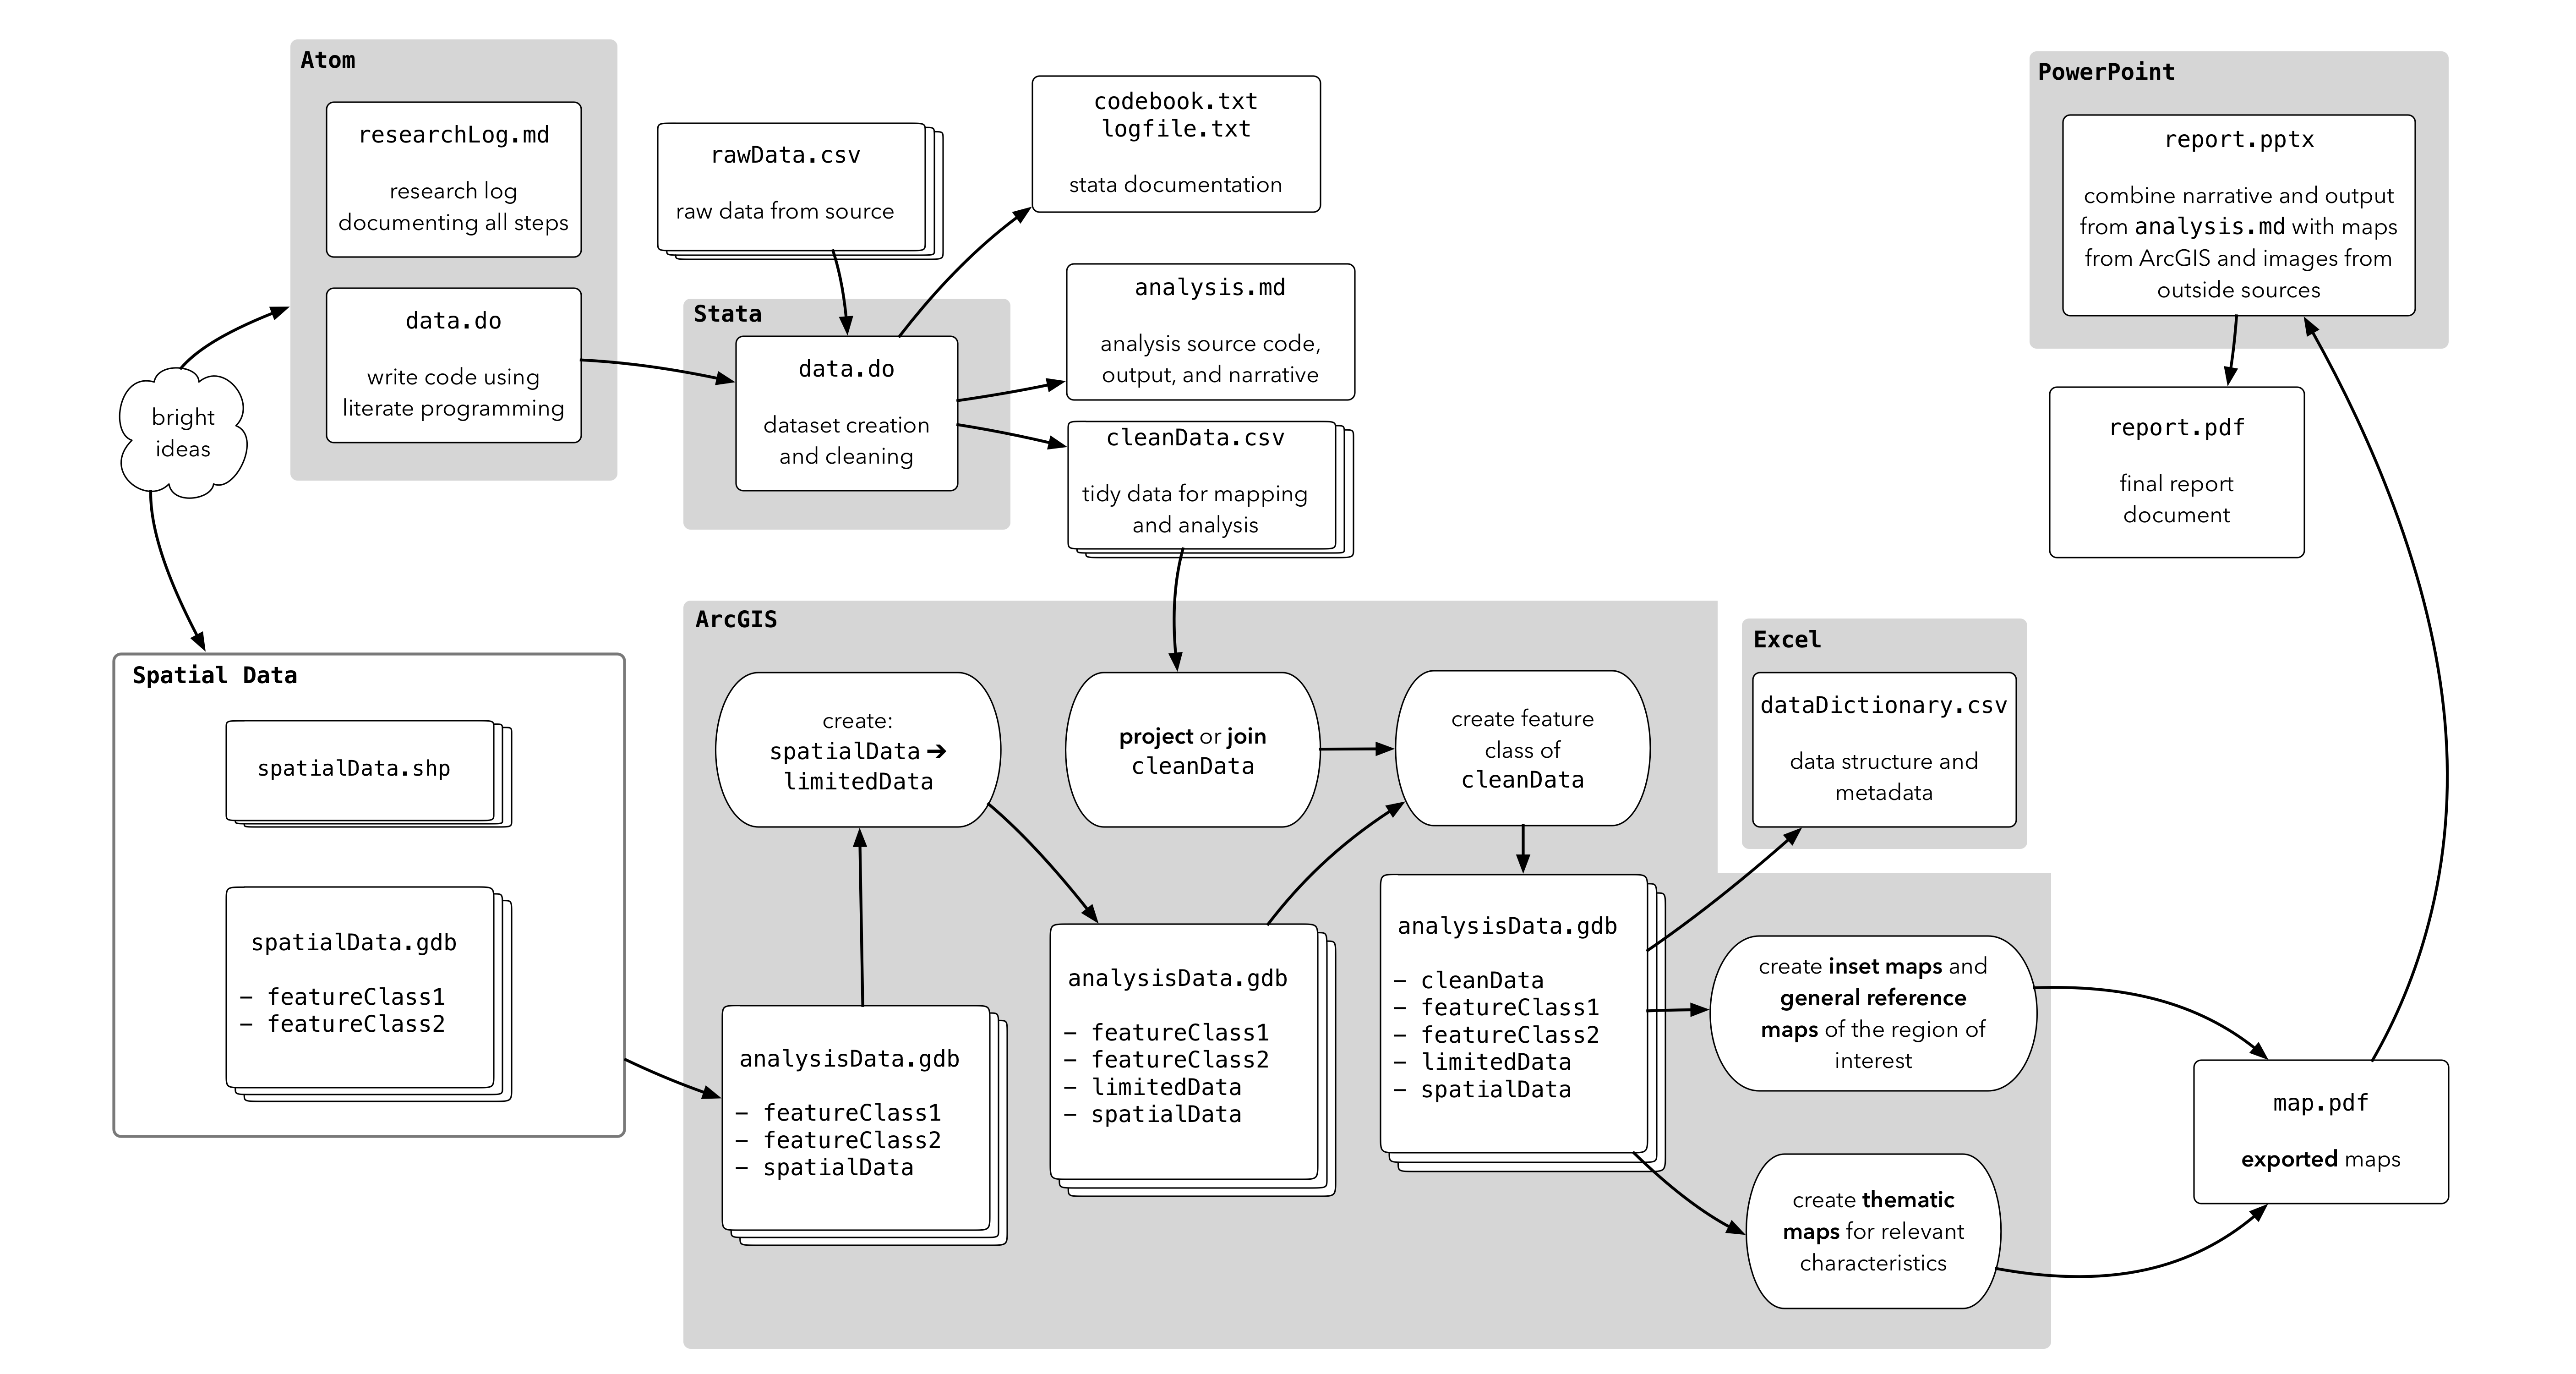
\includegraphics[width=1\linewidth]{images/gisFlow1}

This workflow is premised on a common GISc situation: you have data
stored in some type of database in a \textbf{tabular} or
spreadsheet-like format that have a \textbf{spatial reference} like an
address, which would allow them to be mapped. This main dataset of
interest needs cleaning, as real world data often do, before it can be
mapped. We'll use code written in Atom and executed by Stata to
accomplish this task. We'll also use Atom to maintain and edit
documentation that helps you increase the reproducibility of your work.

Once the data are cleaned, we'll want to start working on mapping them.
This cannot occur in a vacuum. Rather, you will need to seek out data
sources that describe the physical or human geography in the area of
interest. These may come as \textbf{shapefiles} or
\textbf{geodatabases}, and they may also require some sort of data
cleaning. Often the spatial data we have access to cover a larger area
than what we need, or they cover too small an area and have to be merged
with other files to capture the extent we require.

Once both our tabular and spatial data are cleaned, we can bring our
tabular data in ArcGIS so that we can further clean it, if necessary,
and map it. When we have maps ready for export, we often combine them
into deliverables like presentations or printed booklets. This is best
accomplished outside of ArcGIS in an application like PowerPoint or
Word, or a more advanced publishing tool.

Finally, as we noted above, we will capture and track \emph{almost} all
of these files using GitHub:

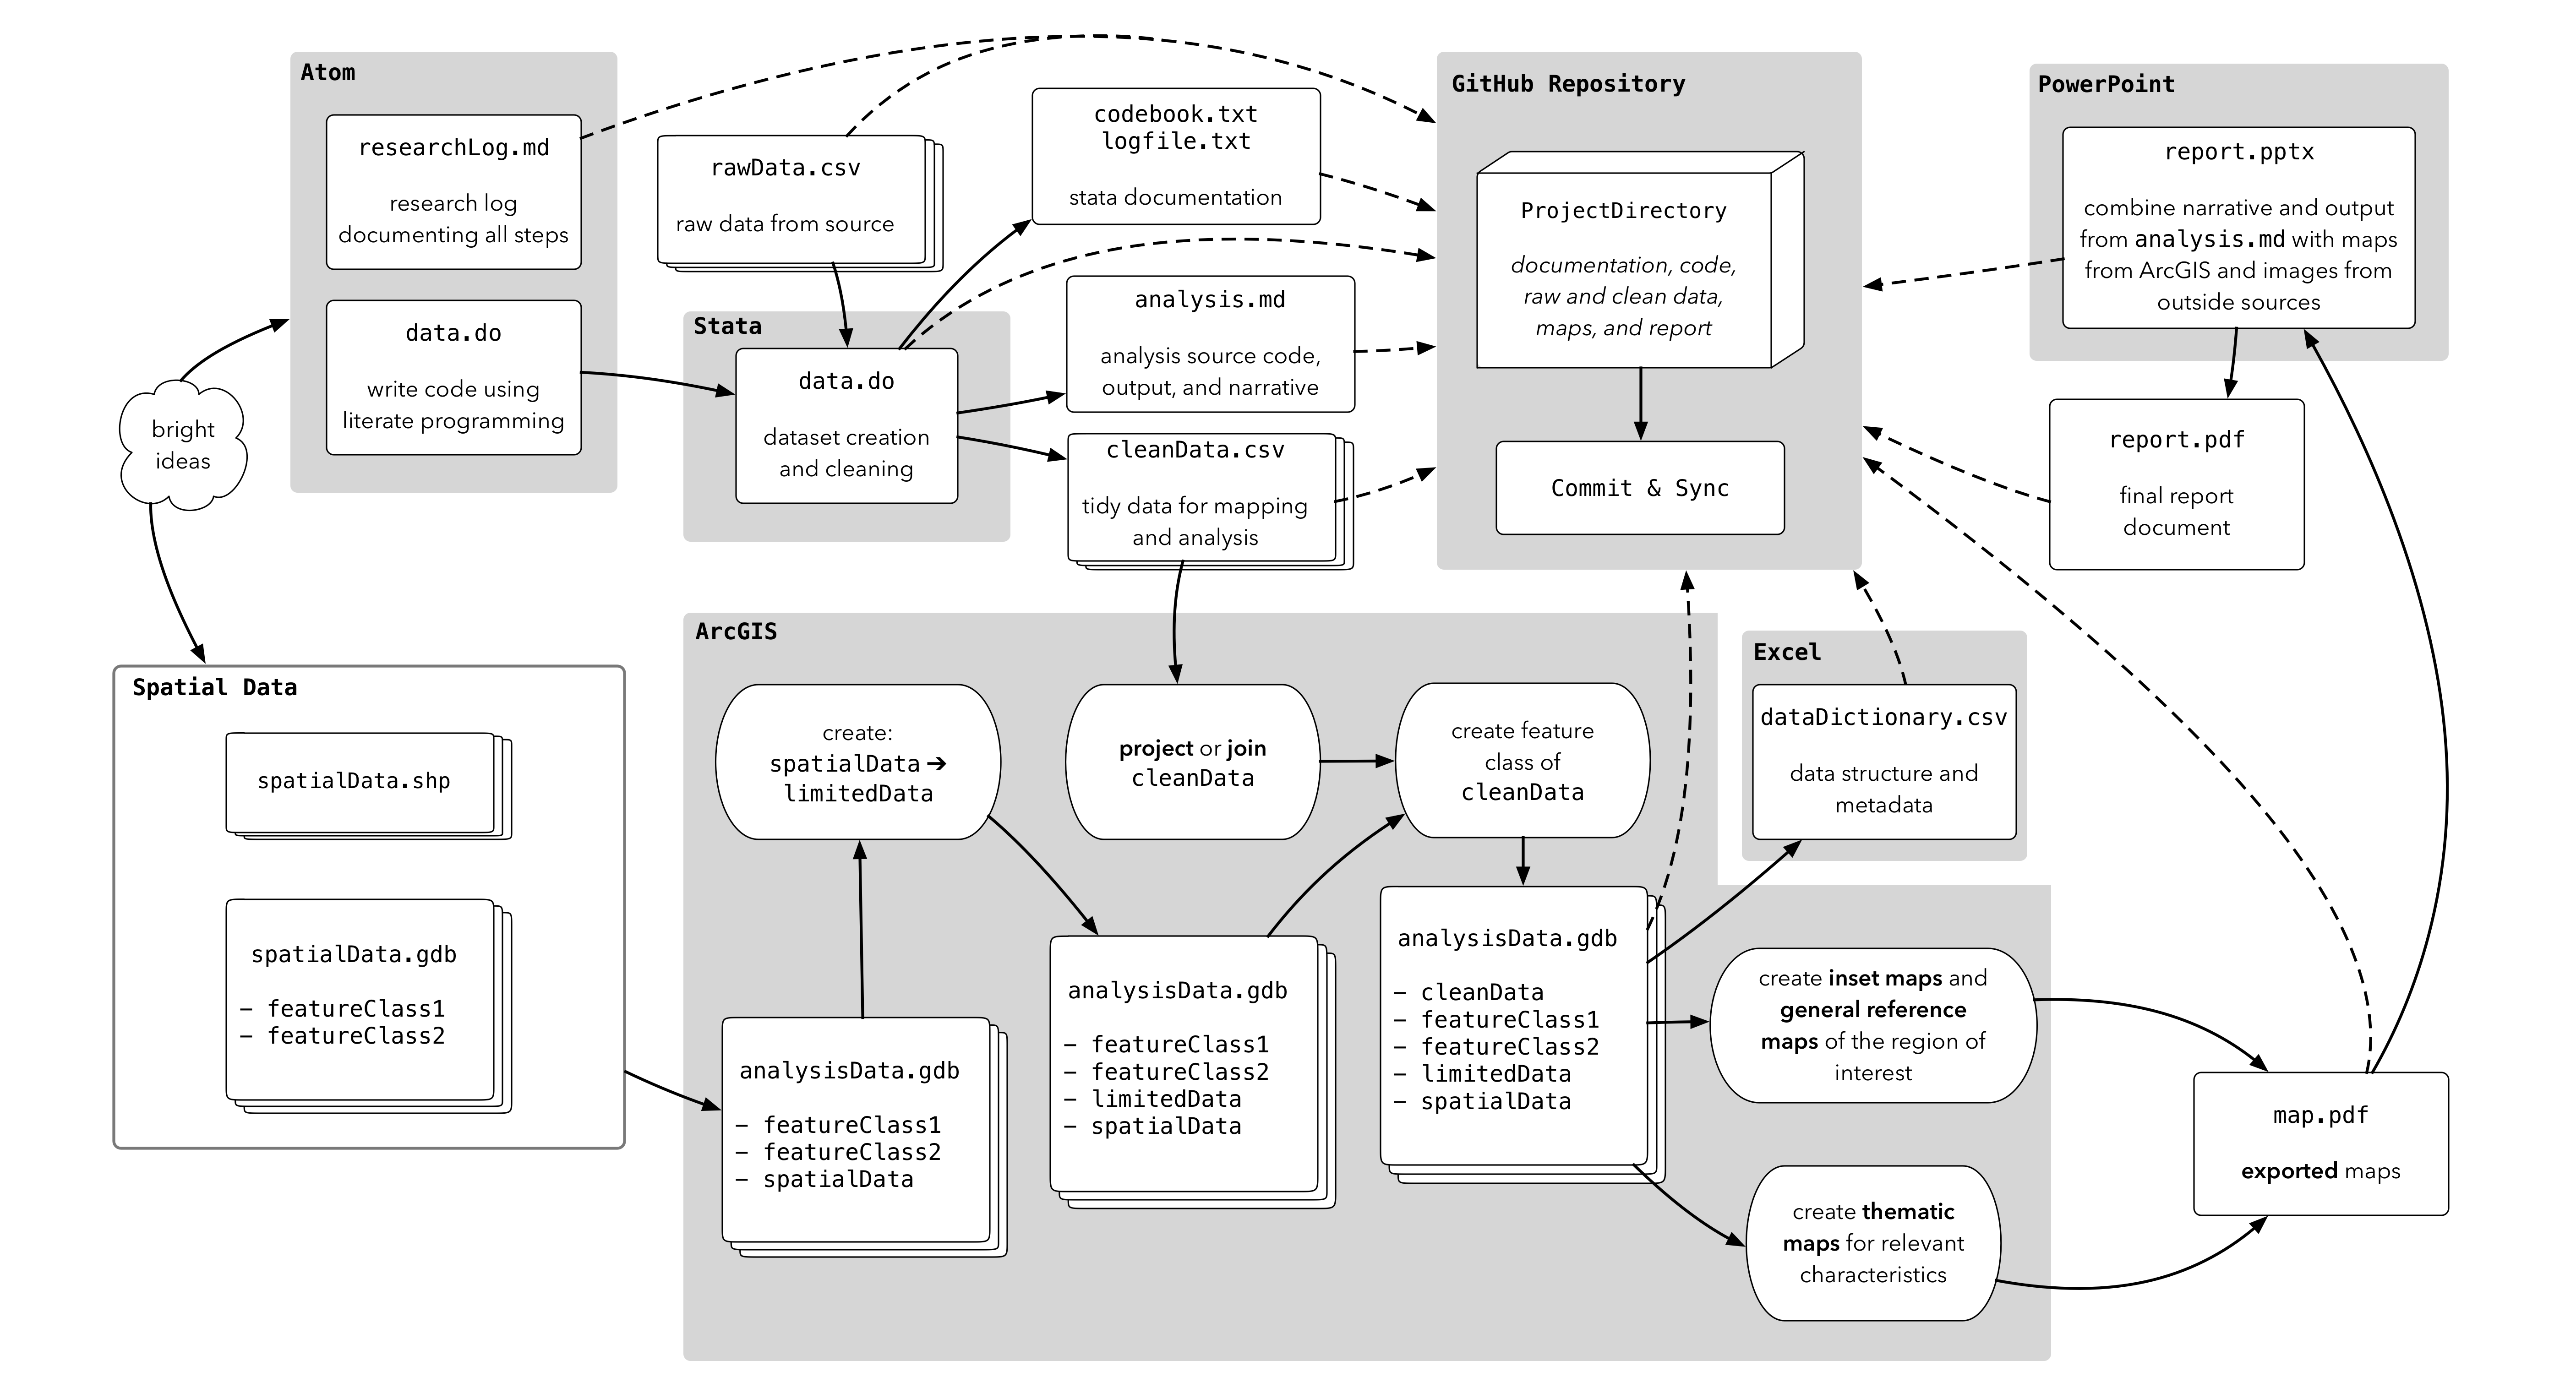
\includegraphics[width=1\linewidth]{images/gisFlow2}

This workflow captures every aspect of a project from the bright idea
that launches it to data acquisition, data cleaning, mapping,
dissemination, and archiving.

\chapter{Protecting Your Work}\label{protecting-your-work}

Each semester that I teach this course or
\href{https://slu-soc5050.github.io}{SOC 5050 (Quantitative Analysis)},
two things happen. The first thing that happens is that students
regularly lose files. The effects of losing files can range from being a
minor frustration to a major headache depending on the file in question.
Losing files often results in downloading multiple copies of the same
data and recreating work. Both of these are wastes of your time.
Moreover, files are rarely gone. They are typically just misplaced. This
is bad for reproducibility, particularly when you happen across multiple
versions of the same file and have to sort out which version is the
version you last worked on.

The second thing that happens is that students lose their thumb drives.
Depending on the timing of this loss, this can again range from being a
minor frustration (very early in the semester) to being downright
anxiety attack producing (last few weeks of the semester). Recreating an
entire semester's worth of work on the final project is both a
tremendous waste of your time and a particularly unpleasant experience.

Fortunately, I have never had a student's computer hard drive die during
the course of the semester. However, I assume that if I teach this
course long enough a hard drive failure will indeed occur. The backup
provider \href{https://www.backblaze.com/}{Backblaze} has
\href{https://www.backblaze.com/blog/how-long-do-disk-drives-last/}{analyzed}
their own hard drives and found that about 5\% of drives fail within the
first year. After four years, a quarter (25\%) of drives in their data
center fail.

Similarly, it is only a matter of time before a student's computer is
stolen along with all of their hard work. A less likely though still
very plausible scenario involves the destruction of a student's
belongings (computer and thumb drive included) in a fire, car accident,
or natural disaster.

Despite the likelihood that you will at some-point lose a thumb drive
(if not during this semester than sometime down the road) and the near
certainty that your computer's hard drive will eventually fail if a
rogue wave does not get it first, few students and faculty take these
risks seriously. While you cannot prevent many of these things from
happening, I want to suggest to you that you can take some simple steps
to sure that \emph{when} (not if) they happen, you are well prepared to
get back to work with minimal disruption.

\section{Data Management}\label{data-management}

One of the themes in \href{https://arxiv.org/abs/1609.00037}{``Good
Enough Practices in Scientific Computing''}, referenced in the previous
chapter, is an emphasis on data management. One of their core messages
is to ``save the raw data''. In GISc work, the raw data can be expansive
- dozens of shapefiles, tabular files, and associated metadata. These
files often come from disparate sources - city open data sites, the U.S.
Census Bureau, state data repositories, and other federal agencies.
Moreover, GIS data are often updated over time to reflect on-the-ground
changes. Saving the raw data in GISc work therefore means not only
creating a well-organized directory containing \emph{all} of your
original data. It also means logging the source of each file, when it
was downloaded, and (if applicable) a permanent web link to your data
source. For that reason, we'll give you not just the course data but a
read me file and a metadictionary that lists all of the files we've
disseminated to you.

A second message in the paper is to ``create the data you wish to see in
the world''. The authors encourage readers to ``create the dataset you
wish you had received.'' First and foremost, this means using open and
not proprietary data formats. For spatial data,
\href{https://en.wikipedia.org/wiki/Shapefile}{ESRI shapefiles} are
technically proprietary, though their standard is open. This means that
other software applications, like \texttt{R}, QGIS, and even Stata can
read and in some cases write shapefiles. For sharing spatial data, a
better option is the
\href{https://en.wikipedia.org/wiki/GeoJSON}{GeoJSON}, which is a plain
text file format.

Tabular data are best stored as \texttt{CSV} files, which is also a
plain text file format that can be opened by a wide variety of
applications. In contrast, common file formats like Microsoft Excels's
\texttt{XLS} and \texttt{XLSX} are proprietary file packages that cannot
be read as plain text and are therefore less desirable for storing data.

Both tabular and spatial data, in their final forms, should be what we
consider ``tidy data''\footnote{Wickham, H., 2014. Tidy Data.
  \emph{Journal of Statistical Software}, 59(i10).} Tidy data are
defined by a number of common attributes - each column represents a
single variable or attribute and each row represents a single, unique
observation. This arrangement should produce clear, easy to read
datasets that represent a single observational unit.

Tidy datasets also have other characteristics. Variable names should be
short, clear, and self-explanatory (i.e. \texttt{streetAddress} and
\texttt{zipCode} are preferable to \texttt{add1} and \texttt{add2}).
Missing data should be properly declared in a machine-readable format
instead of using a code like \texttt{-1} or \texttt{9999}. Filenames
should also be clear and self-explanatory (i.e.
\texttt{stlouisHomes\_011717.csv} is preferable to \texttt{final.csv}).

\section{Creating a Sustainable File
System}\label{creating-a-sustainable-file-system}

In his excellent document \href{http://plain-text.co}{\emph{The Plain
Person's Guide to Plain Text Social Science}}, Kieran Healy describes
two important revolutions in computing that are currently taking place.
One of them is the advent of mobile touch-screen devices, which he notes

\begin{quote}
hide from the user both the workings of the operating system and
(especially) the structure of the file system where items are stored and
moved around.
\end{quote}

For most users, I would argue that this extends to their laptop or
desktop computers as well. I would venture to guess that the majority of
my students are used to keeping large numbers of files on their desktops
or in an (distressingly) disorganized \texttt{Documents} folder.

For research, particularly quantitative research, such an approach to
file management is unsustainable. It is difficult to produce \emph{any}
research, let alone work that is reproducible, without an active
approach to file management.

\subsection{\texorpdfstring{Create a \emph{Single} Course
Directory}{Create a Single Course Directory}}\label{create-a-single-course-directory}

The most successful approach to organizing files is to identify
\emph{one and only one} area that you will store course files in. Having
files scattered around you hard drive between you \texttt{Desktop}
directory, \texttt{Downloads}, \texttt{Documents}, and a half dozen
other places is a recipe for lost files. It can also add complexity to
the task of backing these files up. I recommend naming this directory
simply \texttt{SOC4650} or \texttt{SOC5650}. This is short, has no
punctuation or spaces (which can create conflicts with software), and
explicitly connects the directory to this course as opposed to other
courses you may take that are also GIS courses (a good reason to avoid
naming the directory \texttt{GIS}!).

\subsection{Approach Organizing
Systematically}\label{approach-organizing-systematically}

Within your single course directory, I recommend following much of
Long's (2009) advice on organization. Approach this task systematically
and mindfully. This approach begins with having a number of dedicated
subfolders within your course directory:

\begin{verbatim}
/SOC5650
  /Core-Documents
  /Data
  /DoeAssignments
  /FinalProject
  /Labs
  /Lectures
  /Notes
  /ProblemSets
  /Readings
  /Software
  /WeeklyRepos
\end{verbatim}

Note again how these directories are named - there are no spaces,
special characters, and the names are deliberately short but specific.
For a directory with two words (\texttt{FinalProject} or
\texttt{ProblemSets}), I use what is known as camelCase to name the file
where the second (any any subsequent) words have their first character
capitalized. You could also use dash-case (\texttt{Core-Documents}) or
snake\_case (\texttt{Core\_Documents}) as a naming strategy. Regardless
of which of these approaches you take, try to use it consistently.

The course data release is embedded in an otherwise empty folder
structure that mirrors this layout. When you download these data and the
accompanying directories, un-zip them and move the entire contents to
the root of your thumb drive or external hard drive. If you are
registered for SOC 4650 and want your directory to match your
registration, feel free to rename it \texttt{SOC4650}.

\subsection{\texorpdfstring{The \texttt{Core-Documents}
Directory}{The Core-Documents Directory}}\label{the-core-documents-directory}

This directory will \emph{not} be included in the folder structure that
you download along with the course data release. This directory will be
added to your file system during \textbf{Lab-03}, when it is
\textbf{cloned} from GitHub. A cloned directory is one that retains a
digital link to the data stored on GitHub, meaning that it can be easily
updated if changes are made. This will be explained in greater depth in
the next chapter of the User's Guide. \textbf{Do not edit the files in
these repositories.}

\subsection{\texorpdfstring{The \texttt{Data}
Directory}{The Data Directory}}\label{the-data-directory}

The data directory should have copies of all original data and their
documentation. Most of these data are included in the initial data
release, but you will have to add some additional data to this directory
over the course of the semester. The data in this directory should be
used as needed but not altered (one of the of the ``good enough''
research practices from the previous chapter).

\subsection{\texorpdfstring{The \texttt{DoeAssignments}
Directory}{The DoeAssignments Directory}}\label{the-doeassignments-directory}

Like the \texttt{Core-Documents} repository, this will not be included
in the course data release. You will add it to your file system during
\textbf{Lab-03}. It will also have a different name - your last name
instead of `Doe'. Once you add it, it will contain a number of
subdirectories:

\begin{verbatim}
  /SOC5650
    /DoeAssignments
      /FinalProject
        /Documentation
        /Memo
        /PosterDraft
        /PosterFinal

      /Labs
        /Lab-01
        ...
        /Lab-16

      /ProblemSets
        /PS-01
        ...
        /PS-10
\end{verbatim}

The \texttt{FinalProject} directory contains submission folders for each
component of the final project. If you a registered for SOC 4650, your
directory will look like what appears above. Students registered for SOC
5650 will have three additional subfolders for deliverables related to
the final paper element of the course.

The \texttt{Labs} and \texttt{ProblemSets} directories have subfolders
dedicated to the 26 individual assignments you'll have to submit over
the course of the semester. \textbf{These directories are intended to
store only the deliverables that are requested in each assignment's
directions.} All other files related to each assignment should be stored
elsewhere in your folder structure.

\subsection{\texorpdfstring{The \texttt{FinalProject}
Directory}{The FinalProject Directory}}\label{the-finalproject-directory}

The final project directory should be a microcosm of the larger
directory structure, with most major directories replicated so that your
final project files have a dedicated, organized home:

\begin{verbatim}
  /SOC5650
    /FinalProject
      /Data
      /DataAnalysis
      /Documentation
      /Memo
      /Notes
      /Poster
      /Readings
\end{verbatim}

You'll notice that there are a number of new directories dedicated to
specific aspects of the project.

\emph{SOC 5650 students}: you will want to add directories for the
\texttt{/AnnotatedBib} and \texttt{/Paper} aspects of the assignment. I
also recommend using some type of bibliography software.
(\href{http://endnote.com}{Endnote}, for example, can be obtained for
free by SLU students). Whatever application you choose, keep its primary
database for your project in the \texttt{Readings} folder along with
copies of all \texttt{.pdf} readings.

\subsection{\texorpdfstring{The \texttt{Labs}
Directory}{The Labs Directory}}\label{the-labs-directory}

This directory contains subfolders for each of the sixteen lab
assignments for this course. Save \emph{all} of the associated materials
for each lab assignment here, including text files, documentation, map
files and output, data tables, and any new data that you are asked to
create and save.

\subsection{\texorpdfstring{The \texttt{Lectures}
Directory}{The Lectures Directory}}\label{the-lectures-directory}

This directory contains subfolders for each of the sixteen weeks of the
course. When we create new data files, make maps, or write code during
lectures, save these documents in the appropriate week's folder.

\subsection{\texorpdfstring{The \texttt{Notes}
Directory}{The Notes Directory}}\label{the-notes-directory}

Use this as a home for course notes.

\subsection{\texorpdfstring{The \texttt{ProblemSets}
Directory}{The ProblemSets Directory}}\label{the-problemsets-directory}

This directory contains subfolders for each of the ten problem set
assignments for this course. Save \emph{all} of the associated materials
for each problem set here, including text files, documentation, map
files and output, data tables, and any new data that you are asked to
create and save.

\subsection{\texorpdfstring{The \texttt{Readings}
Directory}{The Readings Directory}}\label{the-readings-directory}

Use this as a home for \texttt{.pdf} copies of course readings.

\subsection{\texorpdfstring{The \texttt{WeeklyRepos}
Directory}{The WeeklyRepos Directory}}\label{the-weeklyrepos-directory}

Clone each of the weekly repos to this directory, and sync them when
updates are made to ensure you have the latest versions of files.

\textbf{Do not edit the files in these repositories.} If you want or
need to work with them, make a copy and save it into the relevant
assignment directory.

\section{Backing Up Your Data}\label{backing-up-your-data}

There are a number of different ways to think about backing up your
data. The most successful backup strategies will incorporate all of
these elements.

\subsection{Bootable Backups}\label{bootable-backups}

``Bootable'' backups are mirrored images of your \emph{entire} hard
drive, down to temporary files, icons, and system files. With a bootable
backup, you can restore your entire computer in the event of a hard
drive failure or a corruption of the operating system files. They are
named as such because you can plug in the external drive that you are
using for this backup and literally boot your computer up from that
drive (typically a \emph{very} slow process).

These backups are often made less frequently because they can be
resource intensive and it is best not to use your operating system while
creating a clone. They are typically made to an external hard drive,
which is subject to similar failure rates as the hard drives inside your
computer. So bootable drives need to be replaced every few years to
maintain their reliability.

Both major operating systems come with applications for creating clones
of your main hard drive that are bootable, and there are a number of
third party applications that provide this service as well.

\subsection{Incremental Backups}\label{incremental-backups}

Incremental backups are designed to keep multiple copies of a single
file (how often depends on the type of software you use and the settings
you select). These can be used to restore an older copy of a file if
work is lost or a newer file is corrupted.

Apple's TimeMachine is a great example of an incremental backup - when
kept on, it creates hourly backups of files that have been changed,
daily backups for the previous month, and weekly backups for previous
months. Once the disk is full, the oldest backups are deleted. Dropbox
also provides a similar service, retaining all previous versions of
files (and deleted files) for thirty days.

Incremental backups are typically good options for recovering files that
have been recently changed (again, depending on the software you use and
the settings you select). Since they run frequently (every time a file
is changed or every hour, for example), recent changes tend to get
captured. They can be limited in terms of their long-term storage - it
may not be possible to recover older versions of a file past a few
weeks.

They are also not always good solutions for recreating your entire
computer since they do not save all necessary program and operating
system files, and may be cumbersome to work with if you need to recover
a large quantity of files. Like bootable backups, these are typically
stored on external hard drives that need to be replaced on a regular
basis.

In addition to the aforementioned Apple TimeMachine, the Windows OS also
comes with a built-in service for creating incremental backups. Dropbox
is a good option if you have a small number of files, but you may find
the need to upgrade to a paid account if you have a large amount of
data.

\subsection{Cloud Backups}\label{cloud-backups}

Cloud backup services like \href{https://www.backblaze.com}{Backblaze}
or \href{https://www.code42.com/crashplan/}{Crashplan} offer
comprehensive backup solutions for customers. These plans typically
require a monthly subscription fee to maintain access to your backups.
While bootable backups protect against hard drive failure and
incremental backups protect against data corruption, cloud backups
protect against catastrophic events like robberies, fires, and other
natural disasters. A fire or a tornado that affect your house may
destroy your laptop and any external hard drives you use for backup, but
your cloud backup will be unaffected.

\subsection{A Workflow for Backups}\label{a-workflow-for-backups}

Just as we need a workflow for approaching file management, it is also
important to establish a routine for backups. With backups, the most
successful workflows are those that require next to no effort on your
part. If you primarily use a desktop, this can be as simple as leaving
two external hard drives plugged into your computer since most backup
software can be set to run automatically. If you have tasks that require
you to manually do something (plug an external hard drive into your
computer, for instance), create a reminder for yourself on a paper
calendar or a digital calendar or to-do list application.

For this course in particular, it is \emph{imperative} that you backup
the data on your flash drive. A number of possibilities exist for
accomplishing this:

\begin{itemize}
\tightlist
\item
  Keep a local copy of your flash drive's files on your computer.
\item
  Keep a \texttt{.zip} archive of your files in a service like Dropbox
  or Google Drive. (Using a \texttt{.zip} archive will prevent issues
  with your \texttt{.git} repositories.)
\item
  Maintain a second flash drive copies of all of your files.
\end{itemize}

Whatever solution you select, make sure you regularly update your
backup. The more often you keep your backup archive updated, the less
stressful and disruptive losing your drive will be. This will likely be
a manual task, so follow the guidance above about creating a repeating
calendar event or to-do list task reminder.

\chapter{Introduction to GitHub}\label{introduction-to-github}

Much of our interaction this semester outside of class will utilize
GitHub.com (or just ``GitHub''). GitHub is a web service that is a
social network for programmers, developers, data scientists,
researchers, and academics. It is also a tool for collaborating on
projects, especially projects that involve writing code.

We'll use GitHub as an alternative to Blackboard, the \emph{course
management system} that students are typically familiar with. Course
materials will be posted there, and GitHub's features will allow you to
copy them and keep them updated as changes are made. You'll also use
GitHub to submit assignments for grading, and we'll give you feedback
and grades via GitHub as well.

\section{Git}\label{git}

GitHub is a web application that utilizes
\href{https://git-scm.com}{Git}:

\begin{quote}
Git is a free and open source distributed version control system
designed to handle everything from small to very large projects with
speed and efficiency.
\end{quote}

Essentially, Git is a project-wide system for tracking changes to files.
Think of it as Microsoft office's track changes feature on steroids -
every change to every file in a directory (a ``repository'' or ``repo''
in Git-lingo) is tracked. You do no need to host files online to use
Git. If you have a project saved locally (say, a doctoral thesis), you
could utilize Git to version control that project without ever uploading
it to the Internet.

For our purposes, this is just about all you need to know about Git. If
you want to learn more, \href{https://git-scm.com/about}{Git's `About'
page} is a great place to start.

\section{More Git-lingo}\label{more-git-lingo}

Beyond ``repositories'', there are a few additional terms that are
specific to Git and that are helpful to know:

\begin{itemize}
\tightlist
\item
  \textbf{Clone}: Make an identical copy of a repository on your local
  hard drive.
\item
  \textbf{Commit}: Approve any changes you have made to a repository.
\item
  \textbf{Sync}: For cloned repositories, files that have been changed
  need to be synced or \textbf{pushed} to GitHub.com after they are
  committed.
\end{itemize}

\section{GitHub.com}\label{github.com}

GitHub is a web service that can host projects using Git's version
tracking. It is widely used by programmers, software developers, data
scientists, and academics to host and collaborate projects.

GitHub is an excellent way to backup files for a project since you can
``sync'' changes made to a repository up to GitHub's servers. It is also
an excellent way to collaborate on files with colleagues while also
using Git's version tracking. Repositories can be either public (like
all of the repos for our seminar) or private, which means that only
people who have been given access to can view the contents of the repo.
Private repos require an upgraded account, which retails for \$7/month.

Students can get access to GitHub's paid services for free, however, by
signing up for a \href{https://education.github.com}{free student
account}. This will give you access to private repositories for as long
as you are a student.

\section{The Workflow of Git and
GitHub}\label{the-workflow-of-git-and-github}

The typical approach to versioning for many students is manual. For a
hypothetical class response paper, it might look something like this:

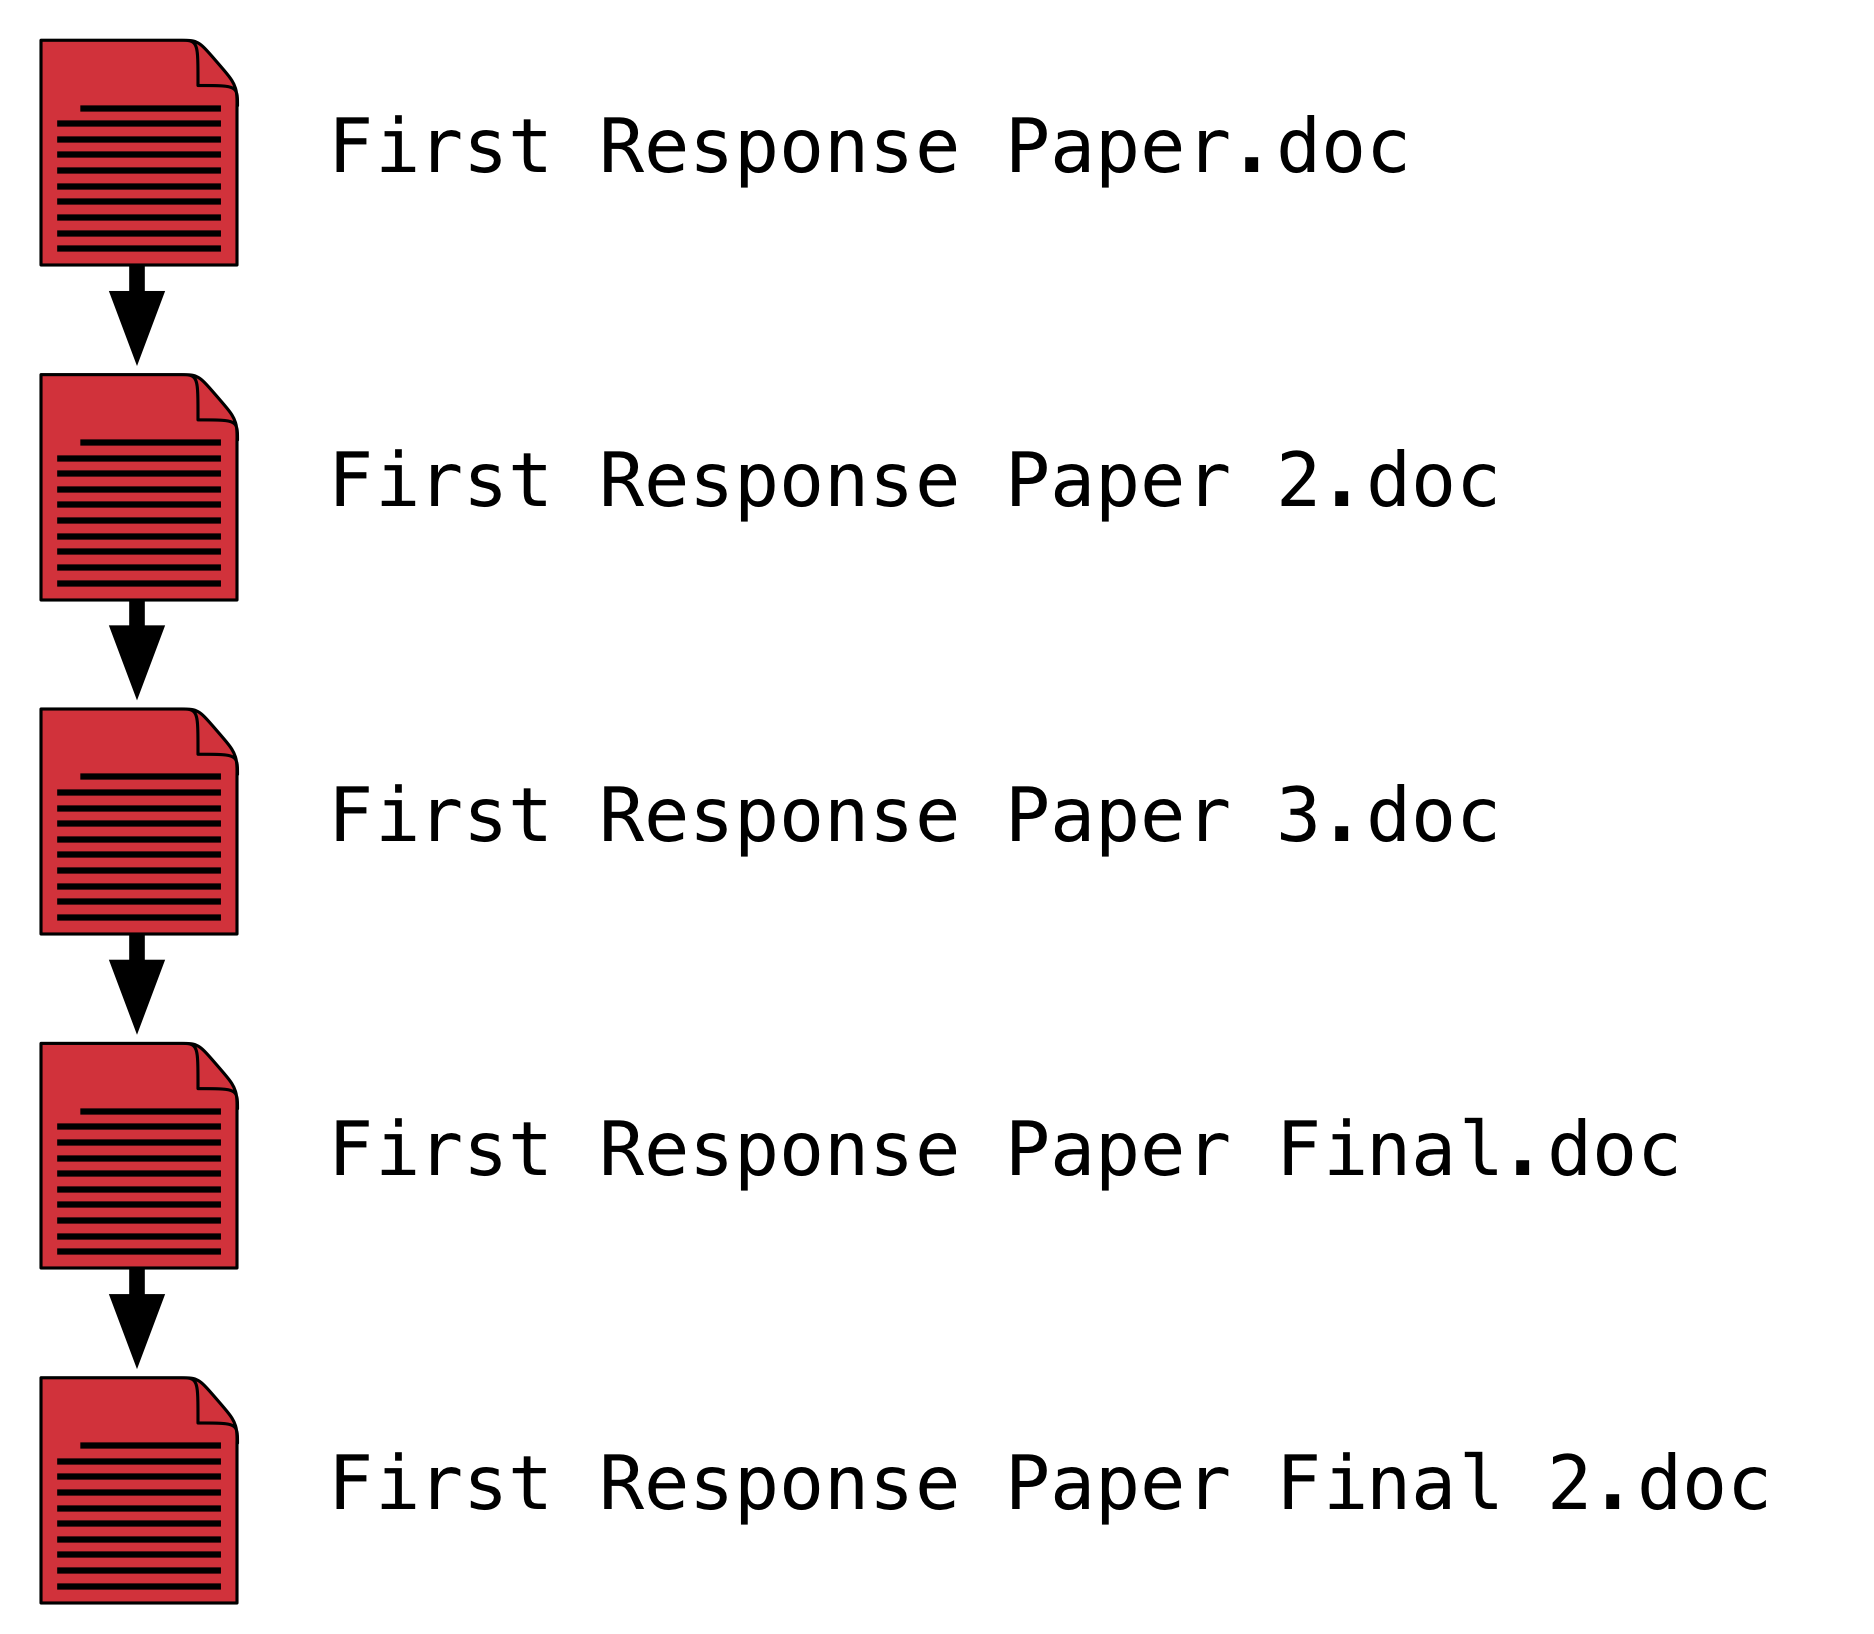
\includegraphics[width=0.5\linewidth]{images/gitFlow01}

The author made an initial copy of the paper, and then used a haphazard
and inconsistent approach for naming subsequent copies of the paper. We
can presume that changes were made in a linear fashion, though it is
easy to make changes to, say, \texttt{First\ Response\ Paper\ 2.doc}
after \texttt{First\ Response\ Paper\ 3.doc} has been created and
edited.

Instead of saving copies of their hypothetical paper, a student using
GitHub could write the paper in a single document, \textbf{commiting}
their changes as they progress to take ``snapshots'' of their progress.
These snapshots contain information on changes the student has made,
tracked line-by-line. So, at each point in which a new document would
have been created in the typical workflow, a student using GitHub would
simply \textbf{commit} their changes:

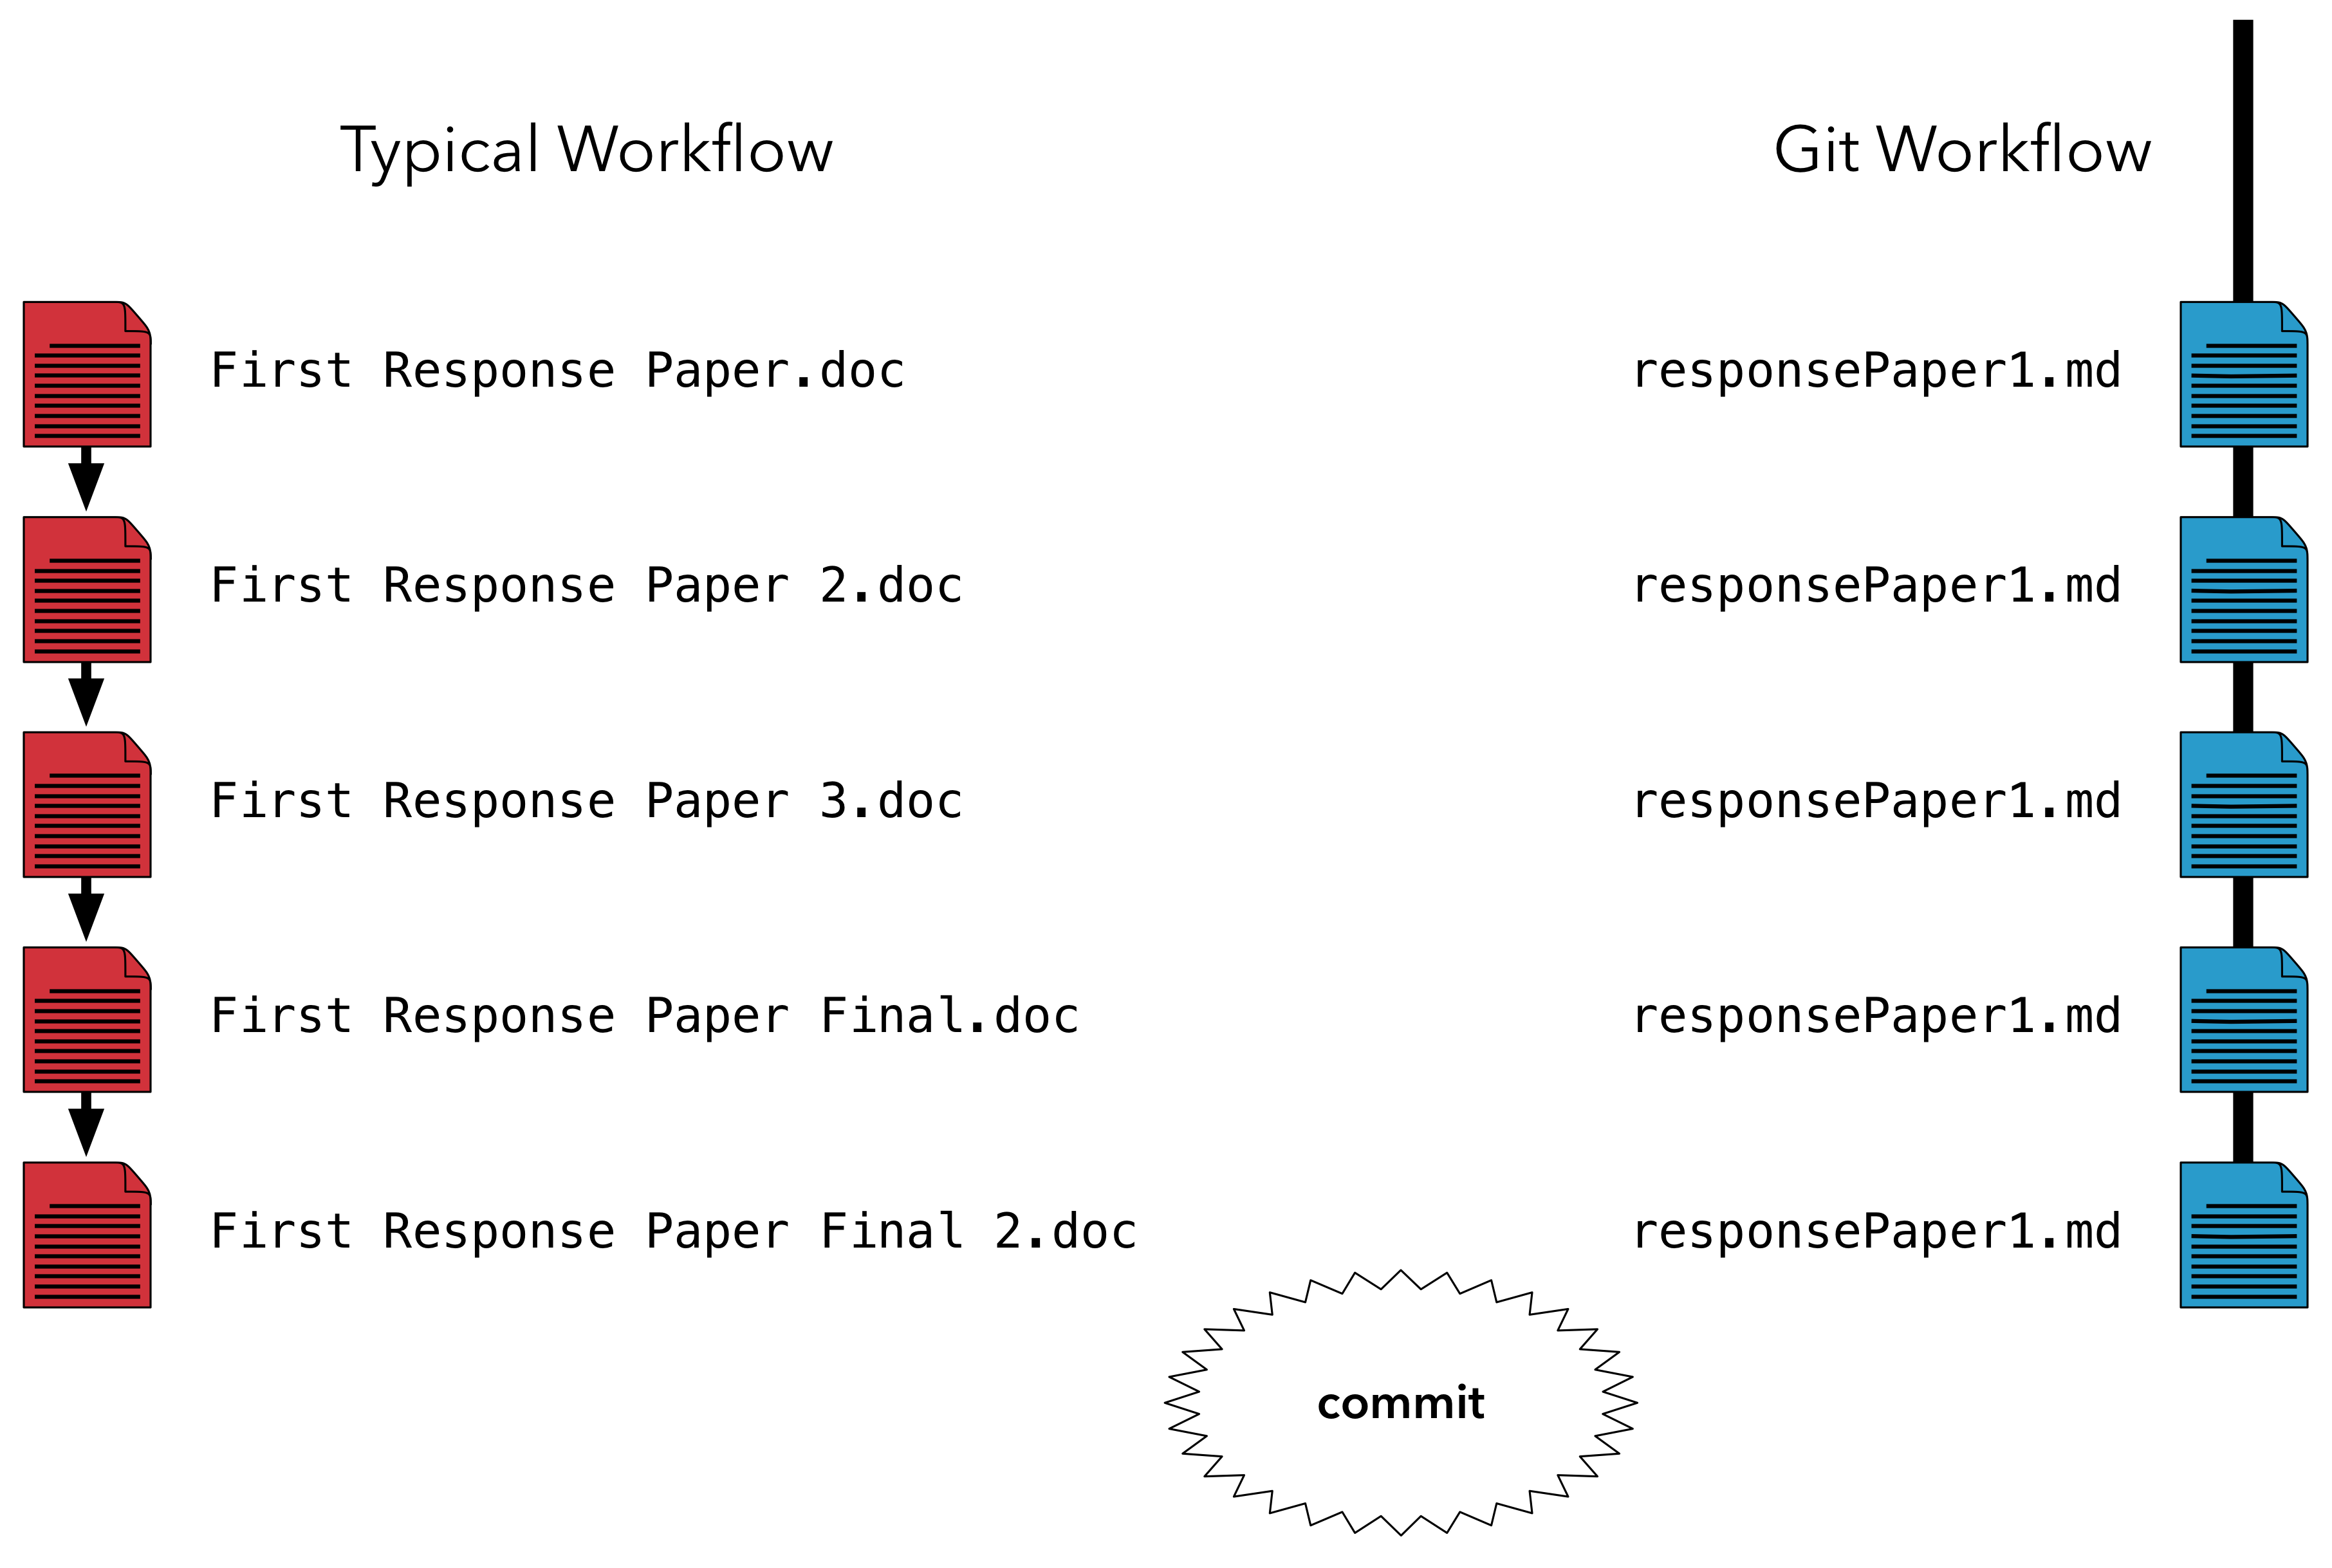
\includegraphics[width=1\linewidth]{images/gitFlow02}

Git provides a number of useful features beyond simply tracking changes.
Each commit is accompanied a \textbf{message}. These messages must have
a short summary that appears on GitHub and can also have a longer
description that can be used to describe in detail what changes are
being applied with a specific commit:

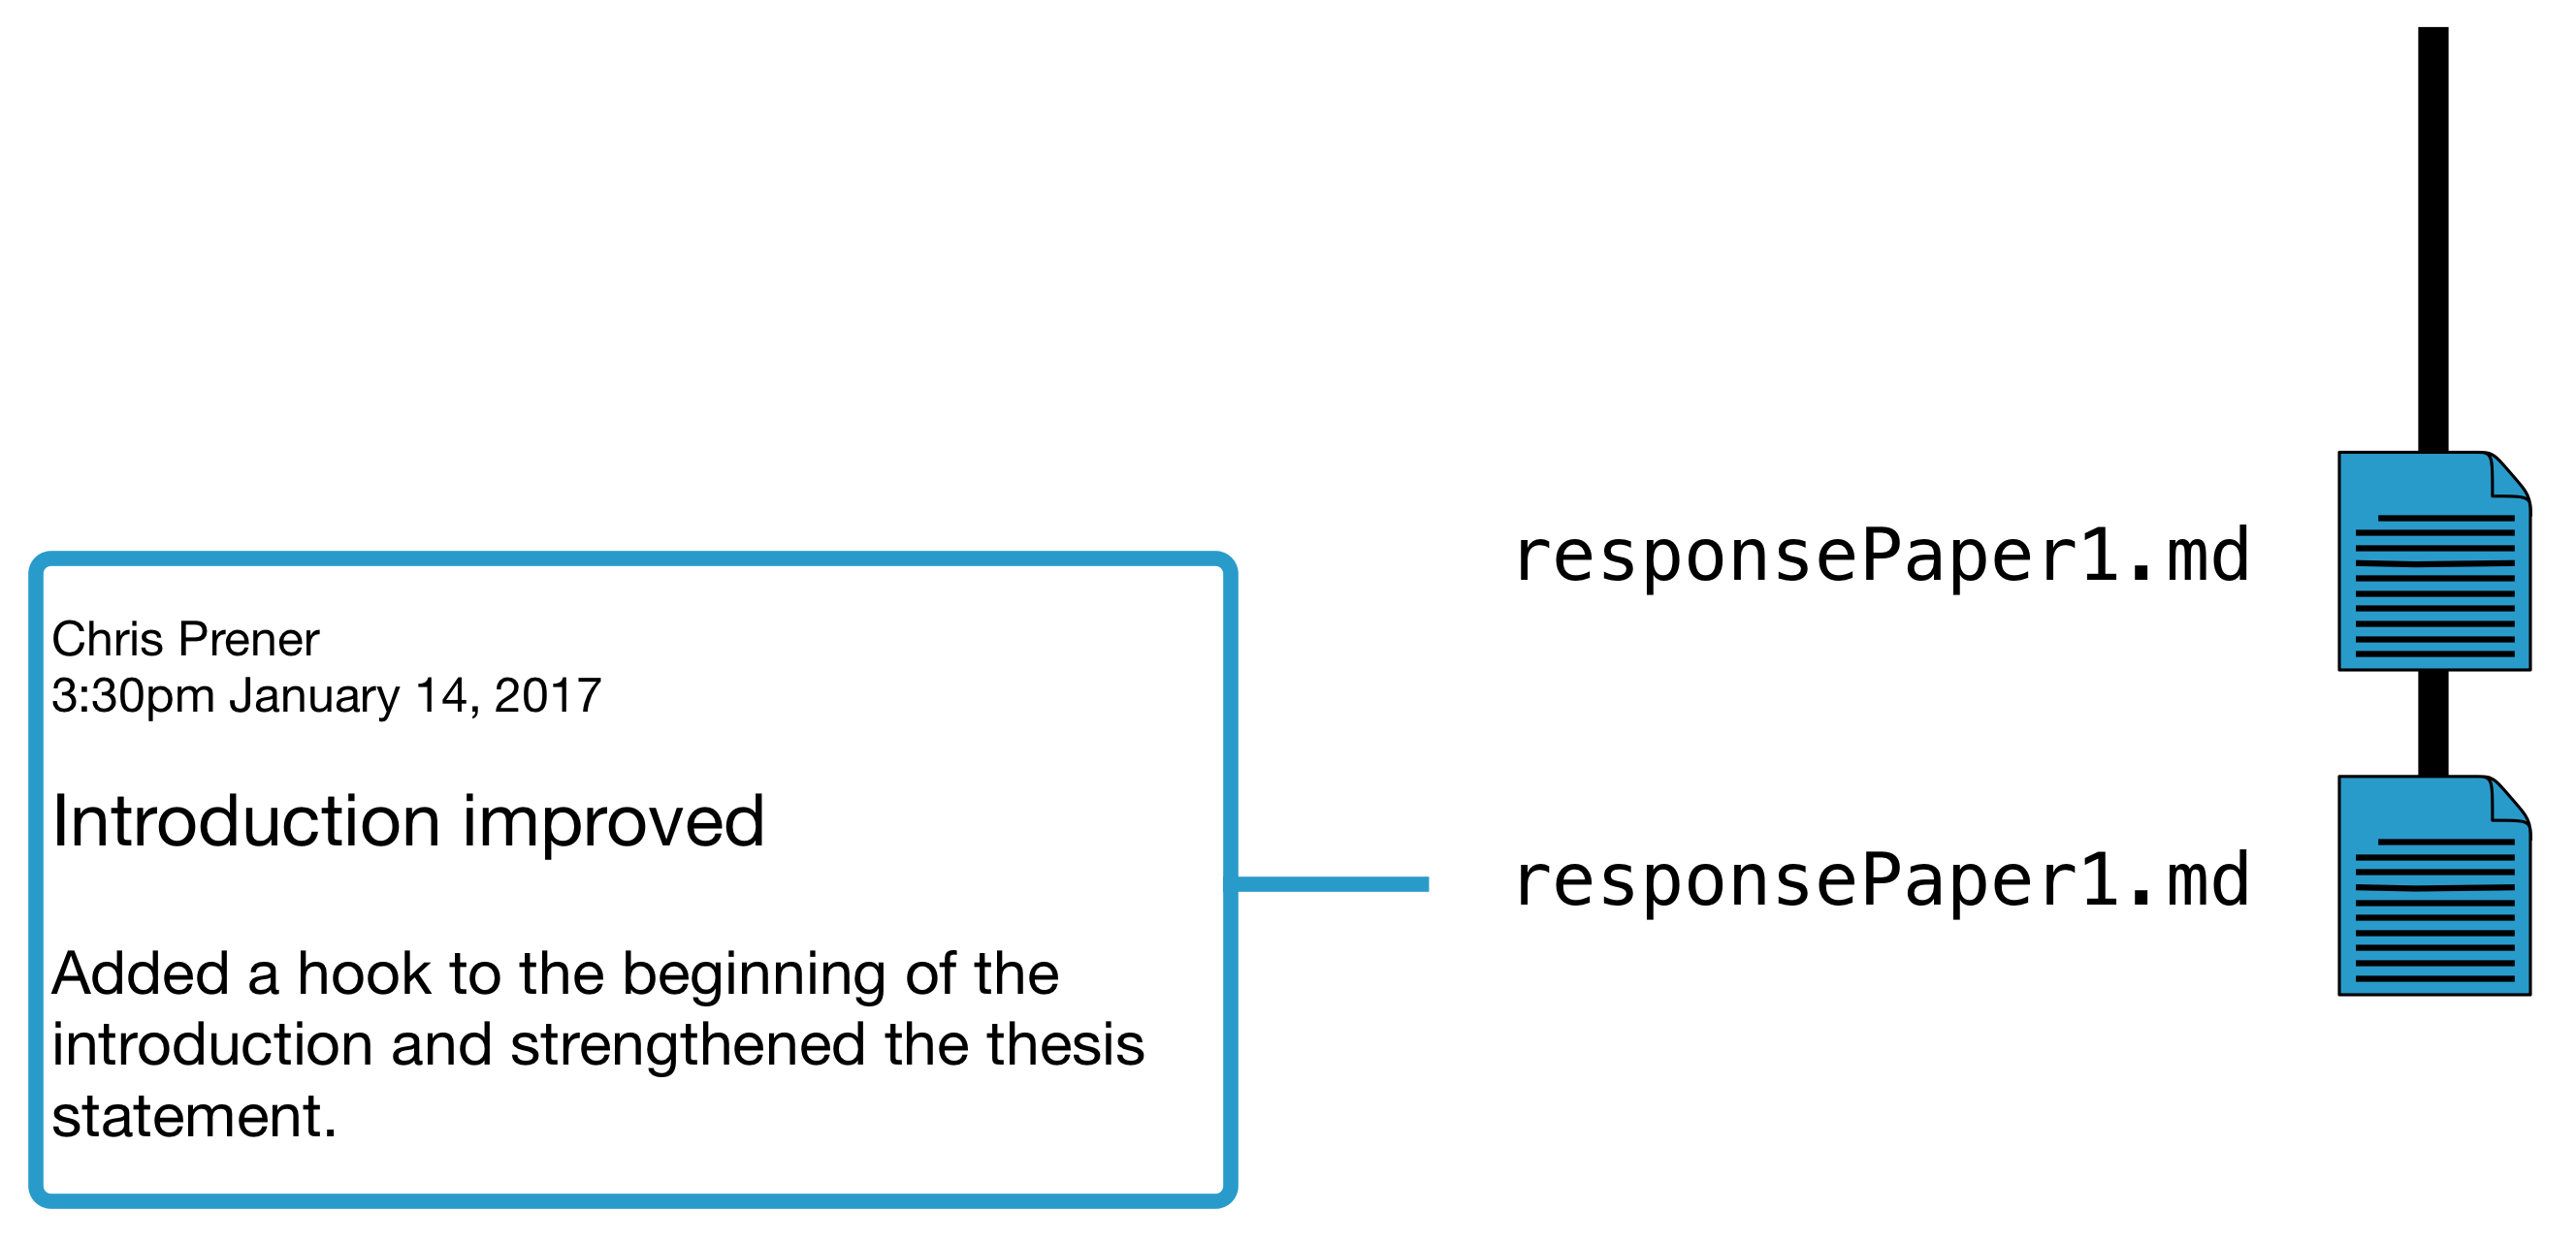
\includegraphics[width=1\linewidth]{images/gitFlow03}

Messages, combined with the changes that are tracked, allow users to
trace the development of a single document or an entire project
overtime:

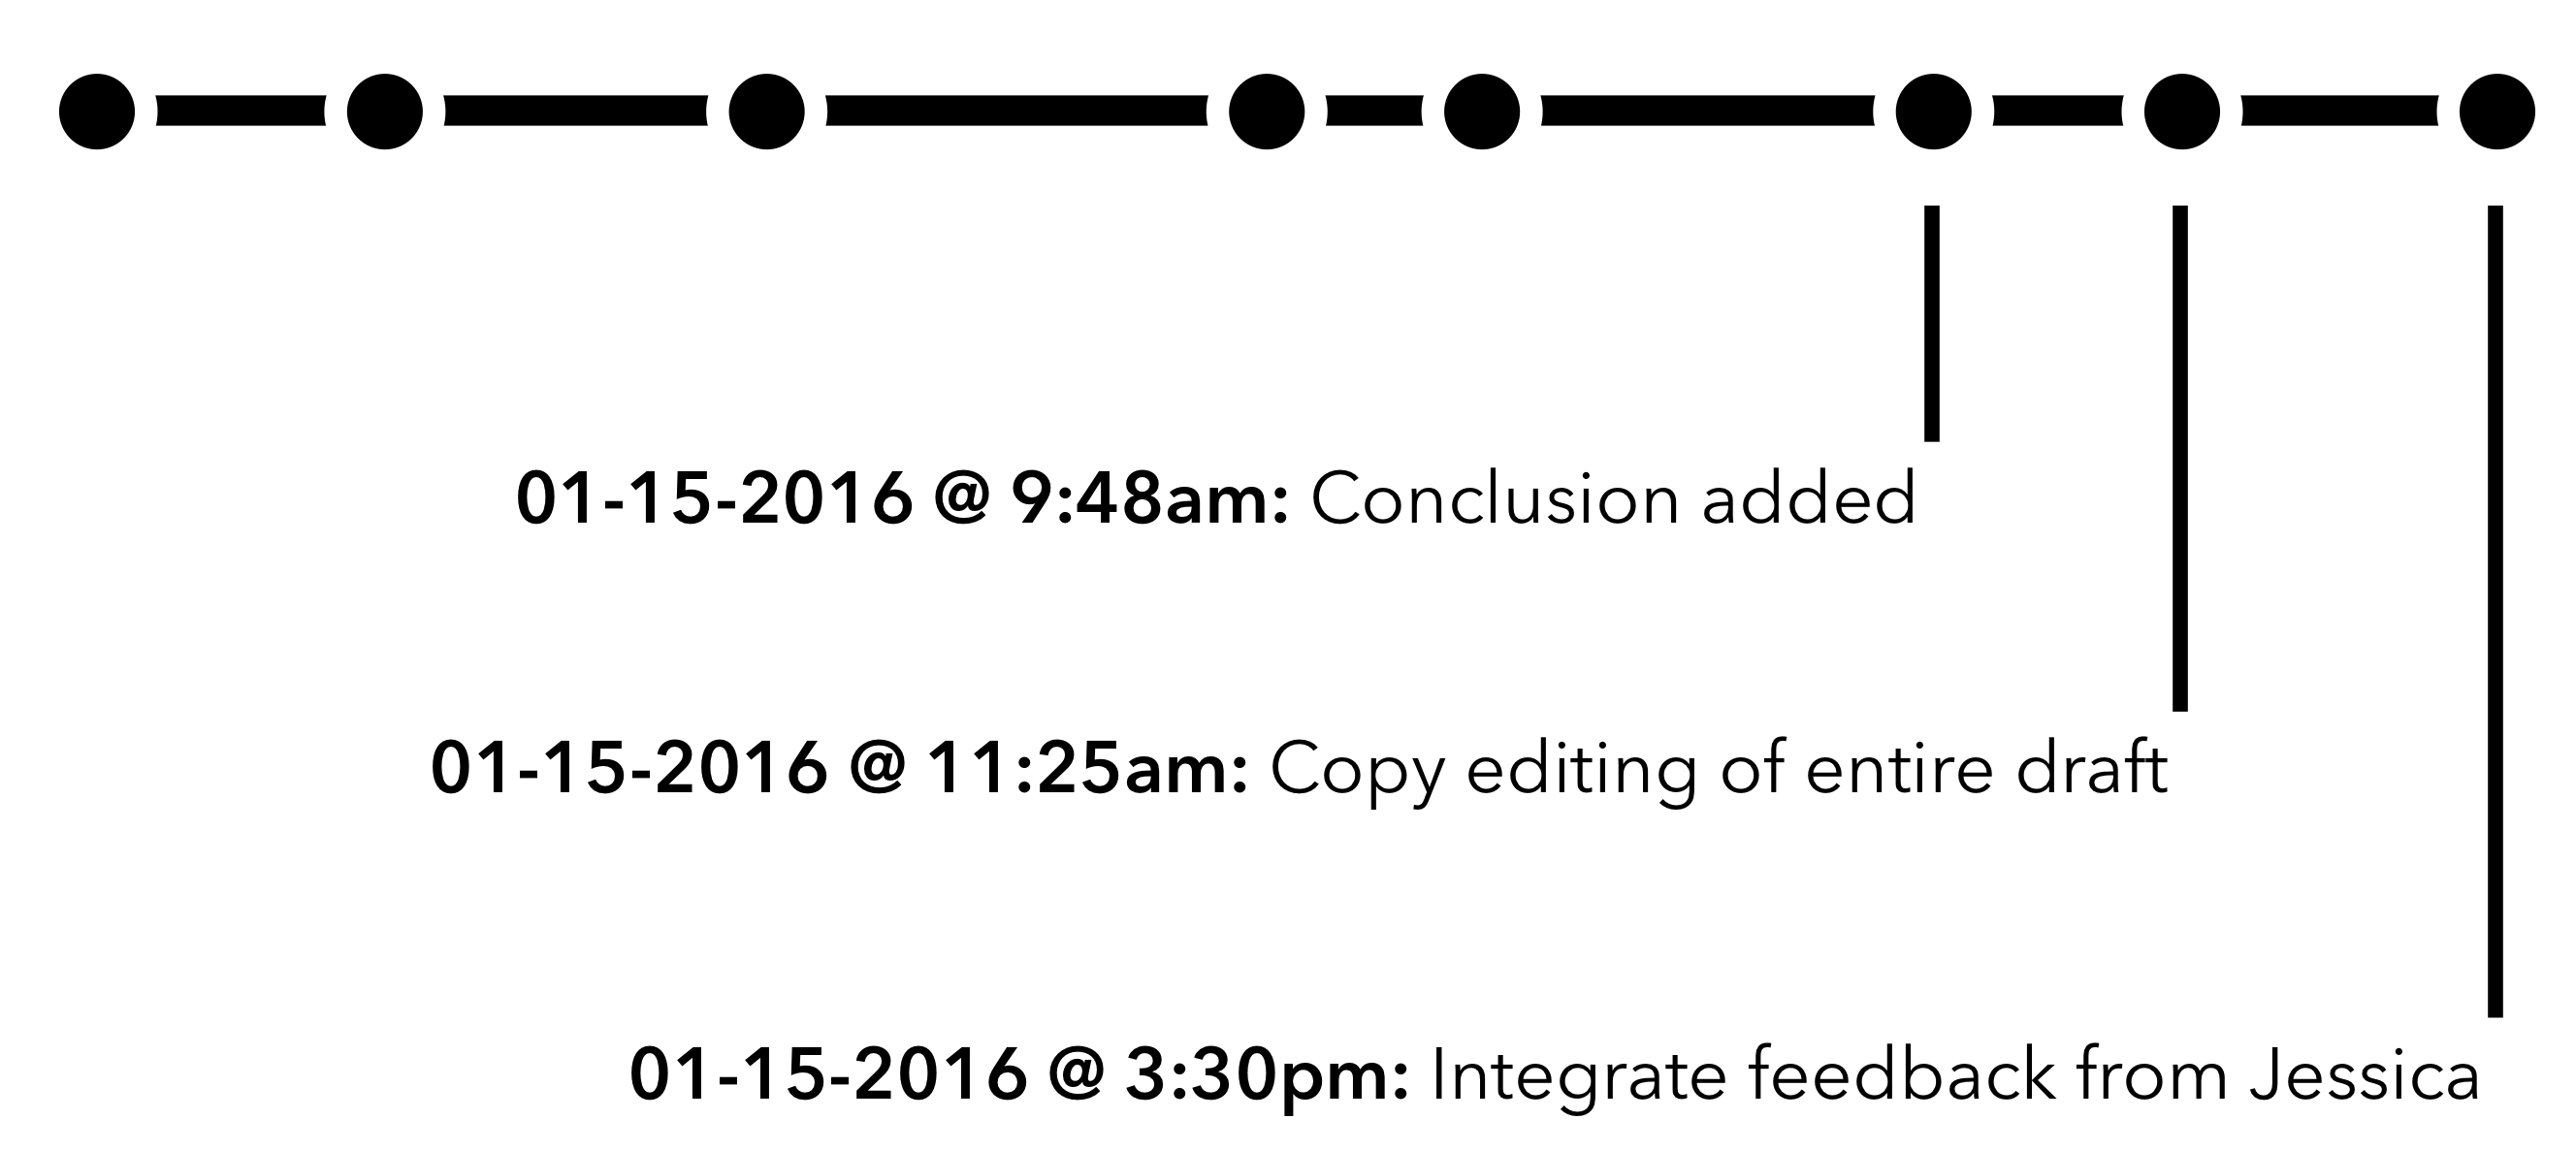
\includegraphics[width=1\linewidth]{images/gitFlow04}

This means that, if necessary, the project can also be rolled back to an
earlier period. Finally, users can \textbf{sync} their commits with
GitHub.com, hosting their changes and their data in a way that protects
them against certain types of computer failures and also allowing them
to easily share their work with others.

\section{GitHub Repositories}\label{github-repositories}

Users of GitHub.com adhere to a couple of norms with their repositories
that are worth knowing about. Repositories cannot have spaces in their
names (much like variables in Stata), so the naming conventions that we
will discuss in relation to Stata this semester all apply to GitHub as
well!

Public GitHub repositories also contain (typically) at least three core
files:

\begin{enumerate}
\def\labelenumi{\arabic{enumi}.}
\item
  A \textbf{license} file - since the data is out there for public
  consumption, it is important to think about how that data is licensed.
  The norm among GitHub users has been to use open source licenses,
  which let others edit and adapt your work. There are a range of
  \href{http://choosealicense.com}{licenses} that are commonly used on
  GitHub.
\item
  A \textbf{README} file - this describes the purpose and content of the
  project.
\item
  A \textbf{.gitignore} file - this stops certain types of files from
  being swept up by GitHub when a user syncs their files with a server.
\end{enumerate}

\section{Storing GitHub Repositories}\label{storing-github-repositories}

When you clone your repositories, you will be prompted to save them on
your computer. There are a number of ways in which this process can
introduce sources for trouble down the road. The principle way that I
have seen students run into problems with GitHub is by storing
repositories on cloud storage services like Dropbox or Google Drive. In
order to avoid any issues, I advise against storing GitHub repositories
in an area of your computer that syncs with a cloud service.

\section{GitHub Issues}\label{github-issues}

GitHub has a powerful tool for interaction called
\href{https://help.github.com/articles/about-issues/}{Issues}. These can
be accessed by opening a repository and then clicking on the ``Issues''
tab. Issues can be ``opened'' by anyone with access to the repository.
They allow for a conversation to occur in the form of messages posted
within the Issue itself. Files can be attached to Issues, and the
messages can contain Markdown formatting. Once the conversation is
complete, issues can be marked as ``closed'', which moves them into a
secondary view on the website so that they are archived.

We'll use issues for both assignment feedback and grading. Please keep
up with issues are they appear, and feel free to follow-up with specific
questions about your grade or the assignment feedback in the Issue
conversation. Once you are satisfied, please mark the issue as closed.

\section{GitHub Desktop Application}\label{github-desktop-application}

\href{https://desktop.github.com}{GitHub Desktop} is a tool that allows
you to easily clone repositories hosted on GitHub, commit changes to
them, and then sync those changes up to the website. You can also create
new repositories, however this is not task you will have to do this
semester. GitHub Desktop is not a fully functional desktop version of
GitHub. For our purposes, it is important to note that the Desktop
application will not let you easily identify when repositories have been
updated by other users, view Wikis associated with repositories, or view
Issues.

\section{Learning More}\label{learning-more}

GitHub has a
\href{https://help.github.com/articles/good-resources-for-learning-git-and-github/}{resources
page} with links to websites that are great for helping you learn more
about how Git and GitHub work! The next chapter also has some additional
GitHub and Git information.

One particularly great \href{https://try.github.io/}{tutorial} walks you
through the command line process for creating and using a git
repository. Even if you do not want to use Git via the command line, the
tutorial does an \emph{excellent} job of describing the logic and
sequence behind the Git workflow.

\chapter{Introduction to Atom}\label{introduction-to-atom}

\href{https://atom.io}{Atom} is a flexible and simultaneously simple and
powerful text editor. Text editors, unlike word processors, are not full
fleged word processors. They are designed to work with \emph{plain
text}, which is ideal for working with computer code. Plain text is also
ideal from a reproducibility standpoint, because it does not rely on
proprietary file types like Microsoft's Word document.

\section{Packages}\label{packages}

Packages for Atom are user-written programs that extend or expand its
functionality. Atom is designed to be modular and thus can be almost
endlessly customizable through the addition of various packages. When
you open Atom, you can go to the Packages menu and see that some
packages are already installed for you. One of these, \textbf{Markdown
Preview}, is very helpful for getting a sense of what the Markdown
syntax you are writing looks like. We'll come back to that package in
the ``Introducing Markdown'' chapter.

New packages can be added through
\texttt{File\ \textgreater{}\ Preferences}\footnote{For users on macOS,
  you will find the Preferences under the Atom menu.}. The Packages tab
will summarize all of the packages you have currently installed. These
will be segregated between Core Packages, those that power the base Atom
distribution you downloaded, and Community Packages, which are packages
that you choose to install to extend Atom. For most packages, you have
the ability to access their settings and, when necessary, install
updates.

The \texttt{Install} tab will allow you to search for and install those
Community Packages. The following packages will be \emph{required} for
this course:

\begin{itemize}
\tightlist
\item
  \texttt{language-stata}
\item
  \texttt{linter}
\item
  \texttt{linter-markdown}
\item
  \texttt{pdf-view}
\item
  \texttt{tidy-markdown}
\end{itemize}

\section{Languages}\label{languages}

One of Atom's strengths is its ability to accommodate various
programming languages. By default, Atom documents are opened as plain
text files. We'll be using two primary file formats this semester:
GitHub Markdown and Stata. Support for GitHub Markdown is included in
Atom's base distribution. Support for Stata is enabled with the
installation of the \texttt{language-stata} package.

To switch between languages, you can either click on the language name
in the lower righthand corner of the Atom screen. Again, by default,
this will say ``Plain Text'' in a new document:

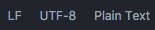
\includegraphics[width=0.35\linewidth]{images/atomLanguages}

Use the search bar that appears to find the desired language, make sure
it is highlighted, and hit Enter to select and switch to that language:

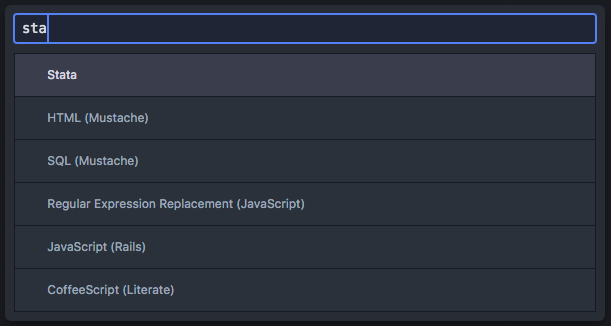
\includegraphics[width=0.75\linewidth]{images/atomLangSelector}

Once you select the language, Atom will provide syntax highlight to
identify distinguishing features of your code, like commands, comments,
and quoted text:

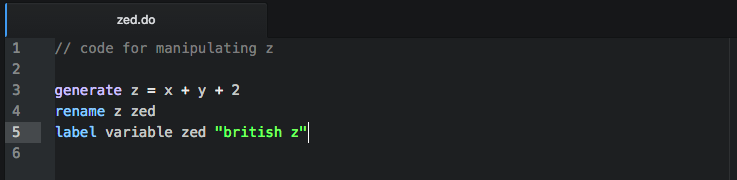
\includegraphics[width=1\linewidth]{images/atomHighlight}

The exact appearance of the highlighting will change based on the theme
that is enabled. These theme selections can be changed under
\texttt{File\ \textgreater{}\ Preferences\ \textgreater{}\ Theme} tab.

When you save files, be sure to include the appropriate \texttt{.do}
file extension for Stata do-files or \texttt{.md} for Markdown files.
When you open files with \texttt{.do} file extensions, Atom will
recognize that they are Stata do-files and automatically change the
language setting to Stata. Likewise, it will recognize and adjust for
Markdown files.

\section{Using Snippets}\label{using-snippets}

One of the advantages of working with Atom is that it has a powerful set
of autocomplete tools. One aspect of these tools are what Atom calls
``snippets''. These are blocks of text or code that can be expanded with
a short trigger phrase called a ``prefix''. The
\href{https://github.com/slu-soc5650/week-02}{\texttt{week-02}}
repository contains a file with several snippets for both Stata and
Markdown files.

\subsection{Installing Snippets}\label{installing-snippets}

To install these snippets, open up the file \texttt{atomSnippets.cson}
in Atom. Then go to File \textgreater{} Snippets. The
\texttt{snippets.cson} file will open. Any valid snippets saved here
will be accessible to you when their associated programming language is
activated in Atom. So, snippets for GitHub Markdown are only available
when GitHub Markdown is selected, and snippets for Stata are only
available when Stata is selected. Copy and paste the contents of
\texttt{atomSnippets.cson} into \texttt{snippets.cson} beginning on a
new line of the file. Save \texttt{snippets.cson}, close all open tabs,
and restart Atom.

\subsection{Expanding Snippets}\label{expanding-snippets}

To use a snippet, you'll want to change the programming language to the
appropriate selection. Begin typing the prefix for your snippet, and a
dropdown menu will appear. For example, typing \texttt{hea} in a Stata
file when you are using our class snippets will bring up the following
options:

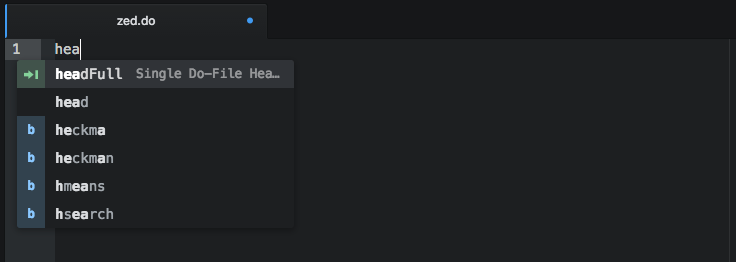
\includegraphics[width=1\linewidth]{images/atomSnippet}

The green arrow icon indicates that the option is a snippet. No icon
indicates that Atom is offering the full spelling of what it thinks is
the appropriate word - ``head'' in this case. The blue ``b'' icon
indicates a possible Stata command (this functionality is only available
when the language is set to Stata).

You can use the up and down arrow keys to select a snippet from this
list. Hit the Enter key for the selected snippet, and the snippet will
expand into your file.

\subsection{Using Tab Stops}\label{using-tab-stops}

Both of the primary snippets for this class include spaces for your to
customize their content after you have expanded them. Once a snippet is
expanded, the cursor will be automatically directed to the first tab
stop. In the Stata snippet, that is a space to give your do-file a
title:

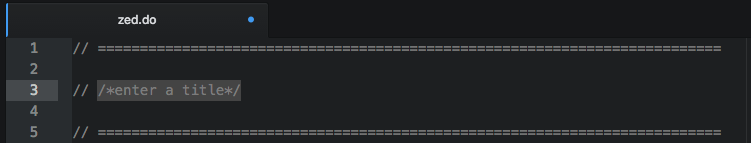
\includegraphics[width=1\linewidth]{images/atomHead}

\emph{Without clicking anywhere} with your mouse, begin typing. Atom
will replace the placeholder text with what you type:

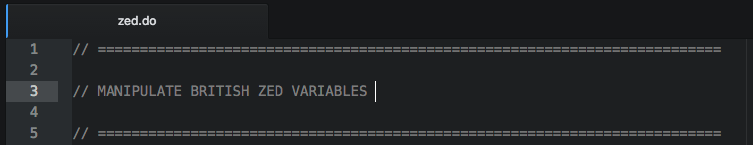
\includegraphics[width=1\linewidth]{images/atomHead2}

When you are done typing, hit the \texttt{Tab} key to be directed to the
next tab stop. Continue typing and using the \texttt{Tab} key to move
through the template.

If you loose the Tab functionality for whatever reason, make sure you
remove the \texttt{/*} and \texttt{*/} fences that sit on either side of
the placeholder text. For Stata in particular, leaving these behind may
cause errors or unexpected output.

\section{Using Panes}\label{using-panes}

Another advantage of Atom is that it allows you to work with multiple
files open at once. This is helpful if you want to place our replication
code side-by-side with your own code, or you want to keep reference
materials close at hand as you write. You can achieve the split screen
effect by right clicking on an open document and selecting Split Right:

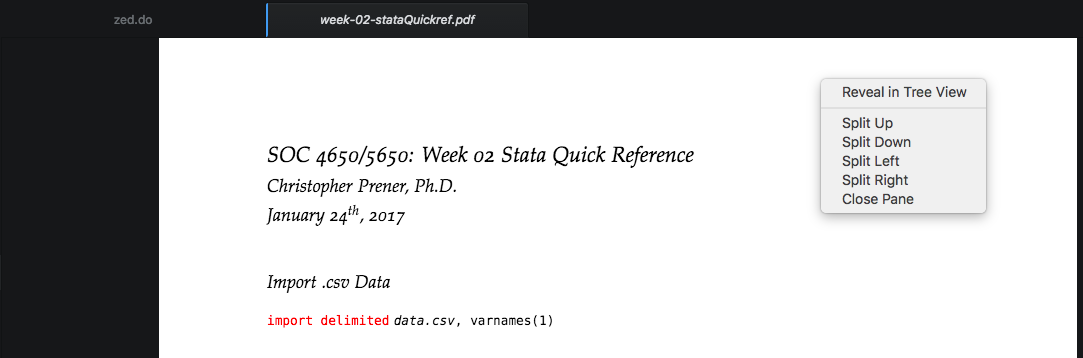
\includegraphics[width=1\linewidth]{images/atomSplit}

After you choose Split Right, you will have two panes displayed side by
side:

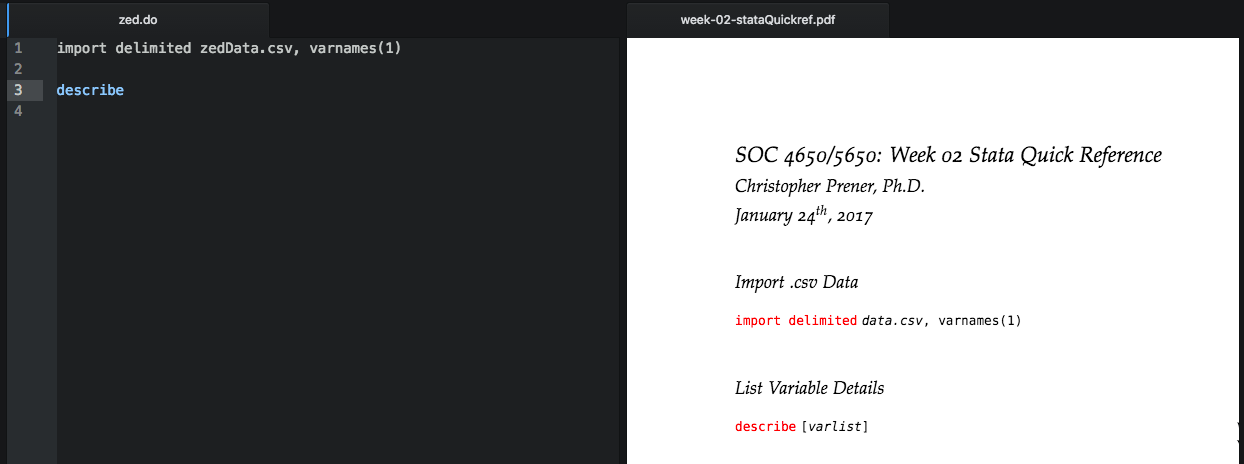
\includegraphics[width=1\linewidth]{images/atomSplit2}

This can allow you to refer to reference material as you write code,
which you may find useful.

\section{Using Project Folders}\label{using-project-folders}

Project folders are directories that you make visible in the
\textbf{Tree View}, the column on the lefthand side of Atom's window.
Directories can be added to the Tree View by going to
\texttt{File\ \textgreater{}\ New\ Project\ Folder...}. Once a directory
has been added, you have full control over its contents. This includes
the ability to drag and drop files into subdirectories, copy and paste
files from one project folder to another, create new files, and create
new subdirectories. Much of this functionality is accessed by right
clicking on the project directory itself:

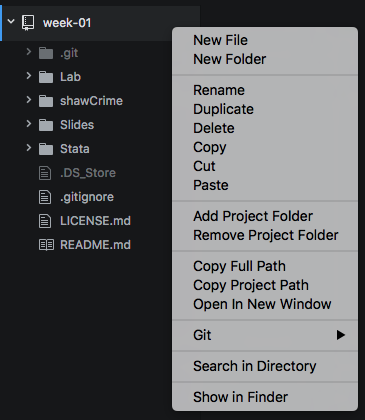
\includegraphics[width=0.75\linewidth]{images/atomProject}

To modify specific files, you can right click on the file itself.

Project folders make it possible to keep a weekly repository, the
assignment directories for that week, and your assignment repository all
close at hand. This will allow you to easily access example and
reference materials, edit assignment files, and copy assignment files
directly into your assignment repository for submission.

\chapter{Reproducible Do-Files}\label{reproducible-do-files}

Do-files are scripts containing Stata code that can be used to execute a
number of Stata commands in order. These provide significant advantages
for researchers, making it easy to edit and adapt data cleaning and
analysis processes. Finding an error in an analysis does not necessitate
recreating hours of work. Instead, do-files allow researchers to quickly
update the source of an error and re-execute the code. A do-file could
be as simple as two lines of code:

\begin{verbatim}
generate z = x + y + 2
rename z zed
\end{verbatim}

Alternatively, large projects may necessitate hundreds or even thousands
of lines of code spread out over multiple do-files.

There are some specific strategies that we can use to make our do-files
serve not just a utilitarian function of executing code but also serve a
larger purpose of increased reproducibility. The Stata snippet that we
are using this semester in Atom is designed to incorporate these
streategies. It will automatically create a series of subfolders in your
working directory that contain a copy of the code you have executed, a
copy of the raw data, a copy of the clean data, the log files, and any
output you create.

The first section of this chapter gives the minimum amount of detail
about using the snippet. The second section describes the process for
``weaving'' code and narrative text. If you want to make sure you are
using the snippet correctly but are less concerned about how all the
code works, just read these two sections.

The subsequent three sections break down the code in the snippet itself.
If you want to know how all the code works, read these sections as well.

\section{Using the Stata Snippet}\label{using-the-stata-snippet}

The Stata snippet in Atom is named \texttt{headFull}. Once you switch a
new document's programming language to \texttt{Stata} and expand the
\texttt{headFull} snippet, you can use the \texttt{Tab} stops to edit
some key aspects of the file:

\begin{itemize}
\tightlist
\item
  line 3 - enter a title for your file - this should be a short, several
  word description that allows you to quickly identify a file's purpose.
\item
  line 9 - enter a project name - this should also be short and should
  not contain any spaces or special characters. Make sure when you save
  your do-file that its filename matches the project name entered here.
  So, for example, if the project's name is \texttt{editZ}, the
  do-file's name should be \texttt{editZ.do}.
\item
  line 44 - enter a title for your analysis - for this class, this will
  most often be something to the effect of ``Lab-01'' or ``Problem Set
  01''.
\item
  line 46 - enter your name
\item
  line 47 - enter today's date
\item
  line 50 - enter a longer description of what this file accomplishes.
  This should describe in detail the goal of this file and what steps or
  tasks it accomplishes.
\item
  line 70 - enter the name of the raw data file \emph{with its file
  extension}. Depending on how long the project description is, this may
  be several lines below line 70.
\end{itemize}

Particularly early in the semester, it may be hard to come up with the
right infromation for some of these prompts. Rememeber to \emph{fully}
read the assignment directions and prompts as you develop a plan for
approaching the assignment. If you do this, you will get a better sense
of the ultimate goal of the assignment and will therefore have an easier
time answering these questions.

As I noted in the ``Introduction to Atom'' chapter, if you lose the
\texttt{Tab} stop functionality, you will need to manually replace the
placeholder text on each of the aforementioned lines. Make sure you
remove the \texttt{/*} and \texttt{*/} fences that sit on either side of
the placeholder text. For Stata in particular, leaving these behind may
cause errors or unexpected output.

When you save your do-file, make sure you save it to the working
directory where you have also copied the raw data and where you plan to
house output created by the do-file.

\section{Weaving Do-files}\label{weaving-do-files}

The workflow described here is largely adapted from the standard setting
\texttt{knitr} package for \texttt{R}.\footnote{See Xie, Y., 2015.
  Dynamic Documents with R and knitr (Vol. 29). CRC Press.} In the
center of the snippet at line 72, you will see this message:

\begin{verbatim}
/* continue adding narrative and code chunks here */
\end{verbatim}

Depending on how long the project description is, this may be several
lines below line 72. This is where you want to begin entering the
commands that are specific to the task you are working on completing.

The \texttt{Markdoc} package, as I have already noted, will combine your
Stata commands, output, and narrative text into a single markdown file.
This ``weaving'' of various sources produces code that can be read and
executed by a computer, but is annotated in such a way that a human can
easily understand its functionality. Narrative text can also be used to
produce a document that purposely links code with output and
description. In essence, you are writing the results section of a paper
along with the code and output that produce it.

A typical combination of these items will look like this:

\begin{verbatim}
sysuse census.dta

/***
**1.** The `sysuse` command opens up pre-installed datasets that come with Stata. 
The `census.dta` file contains demographic characteristics for all fifty states.
***/

summarize pop

/***
**2.** The `summarize` command produces descriptive statistics for the variable 
`pop`. The mean  population for a U.S. state is 4.5 million persons, though there 
is considerable variability between states like Alaska with just over 400,000 persons 
to states like California with over 23 million persons.
***/
\end{verbatim}

Note how the commands precede any narrative text. Also note how
narrative text is wrapped in two ``fences''. These fences, \texttt{/***}
and \texttt{***/}, indicate to \texttt{markdoc} that the text should be
included in the final output.

Once the do-file is fully executed, output will be added to the document
as well:

\begin{Shaded}
\begin{Highlighting}[]

\BaseNTok{          . summarize pop}
\BaseNTok{          (1980 Census data by state)}
\BaseNTok{          }
\NormalTok{**1.** The }\BaseNTok{`sysuse`} \NormalTok{command opens up pre-installed datasets that come with Stata. The }
\BaseNTok{`census.dta`} \NormalTok{file contains demographic characteristics for all fifty states.}

\BaseNTok{          . summarize pop}

\BaseNTok{              Variable |        Obs        Mean    Std. Dev.       Min        Max}
\NormalTok{          -------------+---------------------------------------------------------}
\BaseNTok{                   pop |         50     4518149     4715038     401851   2.37e+07}

\NormalTok{**2.** The }\BaseNTok{`summarize`} \NormalTok{command produces descriptive statistics for the variable }\BaseNTok{`pop`}\NormalTok{. }
\NormalTok{The mean population for a U.S. state is 4.5 million persons, though there is }
\NormalTok{considerable variability between states like Alaska with just over 400,000 persons }
\NormalTok{to states like California with over 23 million persons.}
\end{Highlighting}
\end{Shaded}

To write the narrative correctly, it is necessary to preview the output
by testing commands interactively in Stata until they produce the
desired result. This gives you a chance to test all of your code, which
will cut down on time spent debugging later, but will also give you the
information you need to write the narrative sections.

\section{Snippet Details: Header}\label{snippet-details-header}

The top of the do-file snippet, which we'll refer to as the ``header'',
is designed to create a clean environment for executing code in Stata
and for saving output in your file system. The file begins with the
title block described in the previous section and an area that defines
the ``project name''. This project name is stored in what Stata calls a
\textbf{local macro}, an object that store information that can be
recalled later and utilized. In the snippet, the local macro is named
\texttt{projName}:

\begin{verbatim}
// ==========================================================================

// define project name

local projName "projectName"

// ==========================================================================
\end{verbatim}

The next block of commands is to ensure that there are no holdovers from
previous analyses in your Stata session. Most of these options are
recommended by Long (2009).

\begin{verbatim}
// ==========================================================================

// standard opening options

log close _all
graph drop _all
clear all
set more off
set linesize 80

// ++++++++++++++++++++++++++++++++++++++++++++++++++++++++++++++++++++++++++
\end{verbatim}

The \texttt{log\ close\ \_all} command closes any currently opening
logs, ensuring that your do-file stack does not unintentionally edit any
files. Similarly, the \texttt{graph\ drop\ \_all} closes the graph
window and the \texttt{clear\ all} command clears any other results or
data stored in Stata's memory. The final two commands turn off the
``more behavior'' that limits the amount of output displayed by Stata
(\texttt{set\ more\ off}) and contrains the output width to 80 spaces
(\texttt{set\ linesize\ 80}).

After the environment within Stata is scrubbed, the snippet creates a
series of subdirectories within your working directory.

\begin{verbatim}
// ++++++++++++++++++++++++++++++++++++++++++++++++++++++++++++++++++++++++++

// construct directory structure for tabular data

capture mkdir "CodeArchive"
capture mkdir "DataClean"
capture mkdir "DataRaw"
capture mkdir "LogFile"
capture mkdir "Output"

// ++++++++++++++++++++++++++++++++++++++++++++++++++++++++++++++++++++++++++
\end{verbatim}

You will note that both the \texttt{mkdir} commands here are preceded
with \texttt{capture}. The \texttt{capture} command will suppress any
errors returned by the subsequent command and allow the do-file to
continue executing. Used alone, the \texttt{mkdir} command will generate
an error if a directory already exists with that name.

Finally, the header of the do-file begins logging the do-file's commands
and output. Two log files are created. One is a plain text log file that
is retained as part of your project's documentation. The second is a
specially formatted type of output called a ``smickle'' file. It uses a
special type of Stata syntax called
\href{http://www.stata.com/manuals14/psmcl.pdf}{SMCL} to generate
structured and formatted output.

\begin{verbatim}
// ++++++++++++++++++++++++++++++++++++++++++++++++++++++++++++++++++++++++++

// create permanent text-based log file
log using "LogFile/`projName'.txt", replace text name(permLog)

// create temporary smcl log file for MarkDoc
quietly log using "LogFile/`projName'.smcl", replace smcl name(tempLog)

// ==========================================================================
\end{verbatim}

That package that we will use this semester, Markdoc, relies on the
temporary SMCL log file to generate Markdown formatted output. Notice
that both of these commands refer to the project name \textbf{local
macro} that we created earlier in the file. This is example of recalling
previously stored information. If we wanted to change the name of the
project and were not using a local macro, we would also have to change
these two lines. However, because we used a local macro, changing the
project name on line 9 will automatically result in changes to these
filenames the next time the do-file is executed.

\section{Snippet Details: Body}\label{snippet-details-body}

Once the log files are turned on, everything that is entered will be
passed on to them. In addition to including the basic information like
name, date, assignment, and a description of the code, the do-file
snippet also contains some information about the software dependences
that are required for your code to work.

\begin{verbatim}
### Dependencies
This do-file was written and executed using Stata 14.2.

It also uses the latest [MarkDoc](https://github.com/haghish/markdoc/wiki)
package via GitHub as well as the latest versions of its dependencies:
***/

version 14
which markdoc
which weave
which statax

// ++++++++++++++++++++++++++++++++++++++++++++++++++++++++++++++++++++++++++
\end{verbatim}

The \texttt{version} command signals to Stata that this code was written
for version 14 of the software. When running it under a future release
(such as version 15 or 16), Stata will function as if it were running
the older version 14. The \texttt{which} commands confirm that three
packages are currently installed: \texttt{Markdoc}, \texttt{Weaver}, and
\texttt{Statax}. \texttt{Markdoc} is the main tool that we'll use this
semester to create do-files written in the style of literate
programming. It in turn requires two other packages to function
(\texttt{Weaver} and \texttt{Statax}).

After confirming that all of the necessary dependencies, the do-file
template then uses another \textbf{local macro} to store the name of the
raw data you are working on. As with the project name above, storing the
raw data file's name this way makes editing code easier.

\begin{verbatim}
/***
### Import/Open Data
***/

local rawData "/*enter data file name with extension*/"
\end{verbatim}

After this local, there is space reserved for you to enter your own
commands along with narrative describing their function and their
results. After you have completed this task, the do-file is structured
to save the clean data in two formats: the Stata \texttt{.dta} file
format and as a plain text \texttt{.csv} file.

\begin{verbatim}
// ++++++++++++++++++++++++++++++++++++++++++++++++++++++++++++++++++++++++++

/***
### Save and Export Clean Data
***/

save "DataClean/`projName'.dta", replace
export delimited "DataClean/`projName'.csv", replace

// ==========================================================================
\end{verbatim}

This ensures that your data are ready to be brought into ArcGIS, but you
can also easily pick up editing them in Stata if necessary.

\section{Snippet Details: Footer}\label{snippet-details-footer}

Once the data are saved, it is time to wrap up the do-file's process.
The first task in terms of ending our work is creating the markdown
output that can be posted onto GitHub as part of an assignment's
deliverables.

\begin{verbatim}
// ==========================================================================

// end MarkDoc log

/*
quietly log close tempLog
*/

// convert MarkDoc log to Markdown

markdoc "LogFile/`projName'", replace export(md)
copy "LogFile/`projName'.md" "Output/`projName'.md", replace
shell rm -R "LogFile/`projName'.md"
shell rm -R "LogFile/`projName'.smcl"

// ==========================================================================
\end{verbatim}

The \texttt{markdoc} command takes the SMCL log file and converts its
contents into markdown formatted text containing commands, output, and
narrative text. Once this file is created, it is copied into the
\texttt{Output} directory using the \texttt{copy} command with the
\texttt{replace} option. This option is critical for being able to
re-execute code without returning errors that a file with that name
already exists at the location.

The SMCL log file and the original markdown file that was copied are
then both deleted. It is worth noting that Stata has limited facilities
for deleting content it creates. Its (limited) capacity to delete files
and directories also varies by operating system. In order to accomplish
the deletion of these two files in a way that works on both Windows and
macOS operating systems, we need to invoke the operating system itself
with the \texttt{shell} command. What follows the \texttt{shell} command
in each case is actually an instruction to the operating system itself.
In both Windows and macOS, the \texttt{rm} command with the \texttt{-R}
(recursive) option will permanently delete a file.

With unneeded files removed, we can archive our code and raw data using
the same \texttt{copy} command use above.

\begin{verbatim}
// ==========================================================================

// archive code and raw data

copy "`projName'.do" "CodeArchive/`projName'.do", replace
copy "`rawData'" "DataRaw/`rawData'", replace

// ==========================================================================
\end{verbatim}

After the code are archived, the snippet is structured to close both the
log file and the graph window (if it is open). It also re-sets the
\texttt{more} behavior so that it will occur if Stata is subsequently
used in interactive mode. Finally, the \texttt{exit} command is issued
to explicitly end the execution of the do-files.

\begin{verbatim}
// ==========================================================================
// standard closing options

log close _all
graph drop _all
set more on

// ==========================================================================

exit
\end{verbatim}

\chapter{Introduction to Markdown}\label{introduction-to-markdown}

Markdown is a simple
\href{https://en.wikipedia.org/wiki/Markup_language}{markup language}.
Markup languages are used to give computer programs directions on how
particular blocks of text should be processed. Markdown was developed in
2004 by writer and developer \href{http://daringfireball.net}{John
Gruber}. Gruber describes Markdown on his
\href{http://daringfireball.net/projects/markdown/}{website}:

\begin{quote}
Markdown is intended to be as easy-to-read and easy-to-write as is
feasible.
\end{quote}

\begin{quote}
Readability, however, is emphasized above all else. A Markdown-formatted
document should be publishable as-is, as plain text, without looking
like it's been marked up with tags or formatting instructions. While
Markdown's syntax has been influenced by several existing text-to-HTML
filters --- including Setext, atx, Textile, reStructuredText, Grutatext,
and EtText --- the single biggest source of inspiration for Markdown's
syntax is the format of plain text email.
\end{quote}

\begin{quote}
To this end, Markdown's syntax is comprised entirely of punctuation
characters, which punctuation characters have been carefully chosen so
as to look like what they mean. E.g., asterisks around a word actually
look like \emph{emphasis}. Markdown lists look like, well, lists. Even
blockquotes look like quoted passages of text, assuming you've ever used
email\ldots{}
\end{quote}

\begin{quote}
\ldots{}Markdown's syntax is intended for one purpose: to be used as a
format for writing for the web.
\end{quote}

\section{Markdown Syntax}\label{markdown-syntax}

As markup syntaxes go, Markdown is exceptionally straight forward. The
following sections include examples of syntax used to create Markdown
documents. These are specific to what is called GitHub Markdown - there
are some subtle differences in the way GitHub uses Markdown formatting.

\subsection{Headings}\label{headings}

Markdown contains six heading levels. Headings are identified with
\texttt{\#} symbols:

\begin{quote}
\chapter{This is the largest heading}\label{this-is-the-largest-heading}

\section{This is the second largest
heading}\label{this-is-the-second-largest-heading}

\mbox{}%
\subparagraph{This is the smallest
heading}\label{this-is-the-smallest-heading}
\end{quote}

\subsection{New Paragraphs}\label{new-paragraphs}

Leave a blank line between two lines of text to create a new paragraph.

\subsection{Styling Text}\label{styling-text}

Text can be styled using bold, italics, and strikethroughs. To create
italicized text, wrap your text with a single asterisk \texttt{*\ *}. To
create bold text, wrap your text with double asterisks \texttt{**\ **}.
To create strikethrough text, wrap your text with two tildes
\texttt{\textasciitilde{}\textasciitilde{}\ \textasciitilde{}\textasciitilde{}}.

\begin{quote}
\emph{This is an italicized sentence.}
\end{quote}

\begin{quote}
\textbf{This is a bolded sentence.}
\end{quote}

\begin{quote}
\sout{This is a sentence with strikethrough text}
\end{quote}

\subsection{Quoting Text}\label{quoting-text}

Quoting text (which I have used above to illustrate examples) is done
with a greater then symbol \texttt{\textgreater{}}.

\subsection{Quoting Code}\label{quoting-code}

There are two types of code quotes in Markdown. In-line quotes, which
are included in a sentence, are wrapped in single backticks:
\textgreater{} Use the \texttt{describe} command to list variables in
Stata.

To include code blocks, which are better for including the full syntax
of particular commands and their output, use triple backticks:

\begin{verbatim}
. describe make price mpg

              storage   display    value
variable name   type    format     label      variable label
--------------------------------------------------------------------------------
make            str18   %-18s                 Make and Model
price           int     %8.0gc                Price
mpg             int     %8.0g                 Mileage (mpg)
\end{verbatim}

Note how the word `Stata' is written after the first set of triple
backticks. This is an indicator for GitHub that the code is written in
Stata's programming language. By including this, GitHub can apply some
syntax highlighting to your files. This makes them easier to read.

\subsection{Links}\label{links}

In Markdown, adding hyperlinks is a two step process. The text that you
want to have hyperlinked is written first and is wrapped in brackets
\texttt{{[}{]}}. After this, you include the URL wrapped in parentheses
\texttt{()}. This is an example of including in-line hyperlinks:

\begin{quote}
The course \href{https://github.com/slu-soc5050}{website} is hosted
using the service \href{https://github.com}{GitHub}.
\end{quote}

\subsection{Embedding Images}\label{embedding-images}

Within the directory that contains your Markdown file, create a
subdirectory called \texttt{Output}. Save all images for a particular
assignment there. In your main assignment Markdown file, include a
hyperlink reference:

Note how, instead of including text to be hyperlinked, we suppress this
aspect of the syntax by using an exclamation point \texttt{!}.

\subsection{Simple Lists}\label{simple-lists}

Bulleted lists are indicated in Markdown using the dash \texttt{-} or a
single asterisk \texttt{*}:

\begin{quote}
\begin{itemize}
\tightlist
\item
  mean
\item
  median
\item
  mode
\item
  variance
\item
  standard deviation
\end{itemize}
\end{quote}

Enumerated lists are created by preceding each line with the appropriate
number:

\begin{quote}
\begin{enumerate}
\def\labelenumi{\arabic{enumi}.}
\tightlist
\item
  calculate the mean
\item
  calculate the variance
\item
  calculate the standard deviation
\end{enumerate}
\end{quote}

You can create more complex lists by preceding a line with two single
spaces. You can also combine bulleted and enumerated lists when using
this approach.

\subsection{Task Lists}\label{task-lists}

If you want to create task lists on GitHub, you can include brackets
separated by a space before each list item \texttt{{[}\ {]}}. Completed
tasks include an \texttt{x} in place of the space \texttt{{[}x{]}}.
These task lists are interactive - when published on GitHub, you can
click on the resulting checkboxes to toggle them between complete /
incomplete.

\begin{quote}
\begin{enumerate}
\def\labelenumi{\arabic{enumi}.}
\tightlist
\item
  {[}x{]} calculate the mean
\item
  {[} {]} calculate the variance
\item
  {[} {]} calculate the standard deviation
\end{enumerate}
\end{quote}

\subsection{Mentioning Other GitHub
Users}\label{mentioning-other-github-users}

If you want to mention me or one of your classmates in a comment,
include the \texttt{@} symbol before their username:

\begin{quote}
Hey \citet{chris-prener}, thanks for the feedback. I made the changes to
lines 40 and 41.
\end{quote}

Once the document is uploaded to GitHub, the username will render as a
hyperlink and the user will be alerted.

\section{Markdown and Stata}\label{markdown-and-stata}

\section{Markdown and Atom}\label{markdown-and-atom}

If you write your Markdown documents in Atom, you can use the Markdown
Preview package to generate an interactive preview of your document. As
you type, the preview will update. To open this preview in a tab, go to
\texttt{Packages\ \textgreater{}\ Markdown\ Preview\ \textgreater{}\ Toggle\ Preview}
in Atom.

\bibliography{packages.bib,book.bib}


\end{document}
